\section{Results \& Discussion}

\subsection{\ce{CO2}-Water Mixture}

The phase diagrams of \ce{CO2}-\ce{H2O} mixture at temperatures higher than 420 K is shown in Figure \ref{ELV_CW_Thigh}. The optimized CPA EoS with cross-association captures the trend and shape of the phase diagrams and gives a fair approximation for the critical pressure and composition, which are sensitive to $k_{ij}$. The \ce{CO2} solubility in the aqueous phase is in great agreement with experiments. There are, however, some deviations in the composition of the \ce{CO2}-rich phase at intermediate temperatures ( 423 K $\leq T \leq$ 523 K) and high pressure ($P$ > 500 bar). At such conditions, the only experimental datasets available for the \ce{CO2}-rich phase are from \citeauthor{Tödheide1963} \cite{Tödheide1963} and from \citeauthor{Takenouchi1964} \cite{Takenouchi1964}, and they are in disagreement. Because there is no consensus in the literature on which dataset is more reliable \cite{Liu2011, Zhao2016, Pappa2009, Yang2024}, we adopt both in our CPA EoS parametrization. Our \textcolor{red}{results} lie in between the two datasets, being closer to \citeauthor{Tödheide1963} \cite{Tödheide1963} data at lower temperatures and to \citeauthor{Takenouchi1964} \cite{Takenouchi1964} data at higher temperatures.

\begin{figure}[h!]
\centering
  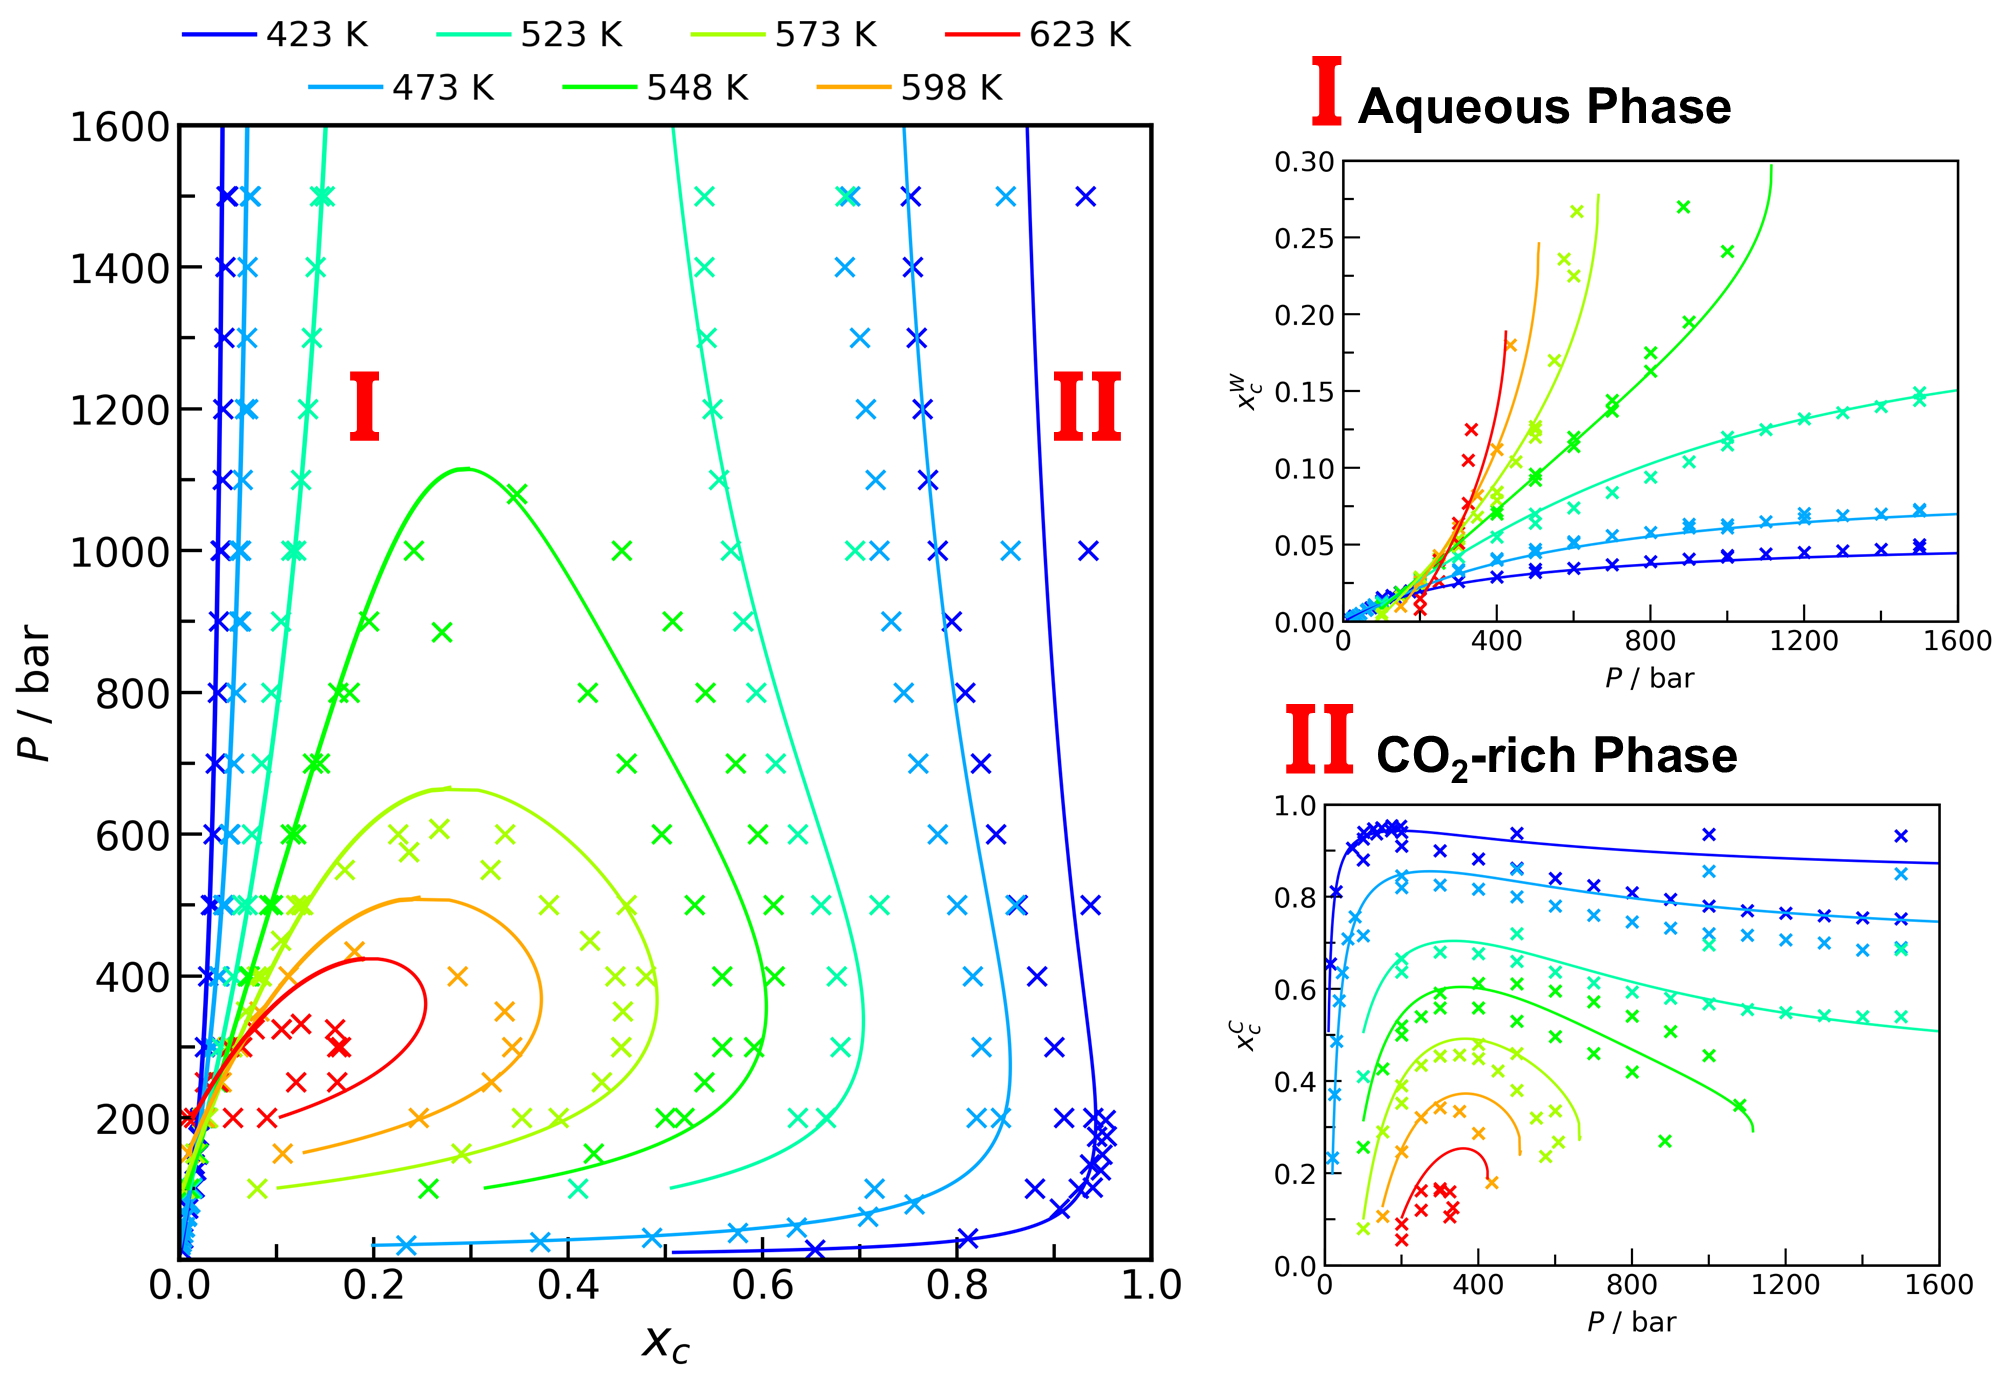
\includegraphics[width=0.95\textwidth]{Figures/ELV_CW_THigh.png} 
\caption{Phase diagram of the \ce{CO2}-\ce{H2O} mixture at high temperature ($T$ > 423 K) from CPA EoS (continuous line) and experiments \cite{Guo2014, Tödheide1963, Takenouchi1964, Sako1991, Hou2013, Nighswander1989, Muller1988} (discrete symbols). The insets (I) and (II) highlight the \ce{CO2} solubility in the aqueous and \ce{CO2}-rich phase, respectively.}
\label{ELV_CW_Thigh}
\end{figure}

Our major focus is on phase behavior modeling at higher temperatures. Nevertheless, our CPA EoS can predict the phase equilibria at temperatures as low as 283 K (Figure S1 from the Supporting Information). The \ce{CO2} solubility in the aqueous phase is predicted with good agreement in the entire range of conditions. \textcolor{red}{At conditions below the \ce{CO2} critical point (304 K, 74 bar), the \ce{CO2}-rich phase is vapor and the phase equilibrium is modeled as VLE. At higher temperatures and pressures, \ce{CO2} is supercritical, the \ce{CO2}-rich phase is liquid-like, and an LLE emerges.} The transition from \textcolor{red}{VLE} to \textcolor{red}{LLE} is not captured by our CPA EoS accurately in the \ce{CO2 }-rich phase at $T$ < 304 K, resulting in larger average deviations in this phase (Table \ref{EXPs_CW}). At temperatures higher than 304 K, the CPA EoS describes the mutual solubility in both phases with good agreement with the experimental dataset. \textcolor{red}{We compute \ce{CO2} Henry's constant in water and compare it with experiments (Figure S2 from the Supporting Information), achieving an average deviation of 24.3 \%. The non-monotonic behavior of \ce{CO2} Henry's constant is captured with a maximum estimated at 430 and 450 K by CPA EoS and experiments, respectively. At higher temperatures, using the Krichevsky-Kasarnovsky equation to interpret Henry's constant may lead to wrong experimental values because the assumption of unity for the solute activity coefficient may no longer be valid.}   

We compare our model (TW) with previous CPA EoS (Figures S3 and S4 of the Supporting Information). The selected models are from \citeauthor{Li2009} \cite{Li2009} with cross-associating \ce{CO2} (RERI), and from \citeauthor{Tsivintzelis2011} \cite{Tsivintzelis2011} with \ce{CO2} as inert molecule (DTU), which is the model used in the eCPA EoS from \citeauthor{Maribo2015} \cite{Maribo2015}. TW and RERI models outperform DTU CPA in the entire range of conditions, indicating the importance of accounting for the cross-association between \ce{CO2} and water. RERI CPA can represent both \textcolor{red}{LLE} and \textcolor{red}{VLE} and may be a better model at low temperatures. At higher temperatures, our CPA model better represents the \ce{CO2}-water phase diagram.

Density is an important property of the \ce{CO2}-water mixture in geological applications. To properly describe the \ce{CO2} migration and fingering effects due to gravity segregation, the model must predict density accurately \cite{Solovsky2025}. Figure \ref{RHO_CW} shows density of aqueous and \ce{CO2}-rich phases in equilibrium. \textcolor{red}{The transition from VLE to LLE is observed from the change in the density slope for temperatures lower than the \ce{CO2} critical temperature}. In the range of 293 — 468 K and 1 — 800 bar, the absolute average deviation of the aqueous phase density is 0.47\%. The \ce{CO2}-rich phase density has deviations at higher pressure. The absolute average deviation in the range of 304 — 478 K and 1 — 1300 bar is 5.33\%. We also compute the aqueous phase density below the \ce{CO2} saturation (295 K < $T$ < 450 K, 150 bar < $P$ < 1000 bar, 0.005 < $x_c$ < 0.03) and compare with experiments \cite{Wright2015} (Figure S5 from the Supporting Information). Different from other gases, \ce{CO2} dissolution in water often increases the mixture density, which induces natural convection and accelerates the convective mixture in CCS formations. Our CPA EoS describes the increase in density with \ce{CO2}, achieving an average deviation of 0.75\% for unsaturated solutions. Overall, our model predicts the density of the \ce{CO2}-water mixture accurately without volume translation parameters and without using density data in the parametrization. To the best of our knowledge, there is no experimental data of the mixture density at temperatures higher than 480 K, but based on the trend with temperature and the phase behavior, we expect a good performance on the density predictions at higher temperatures.   


\begin{figure}[h!]
\begin{subfigure}{.45\textwidth}
  \centering
  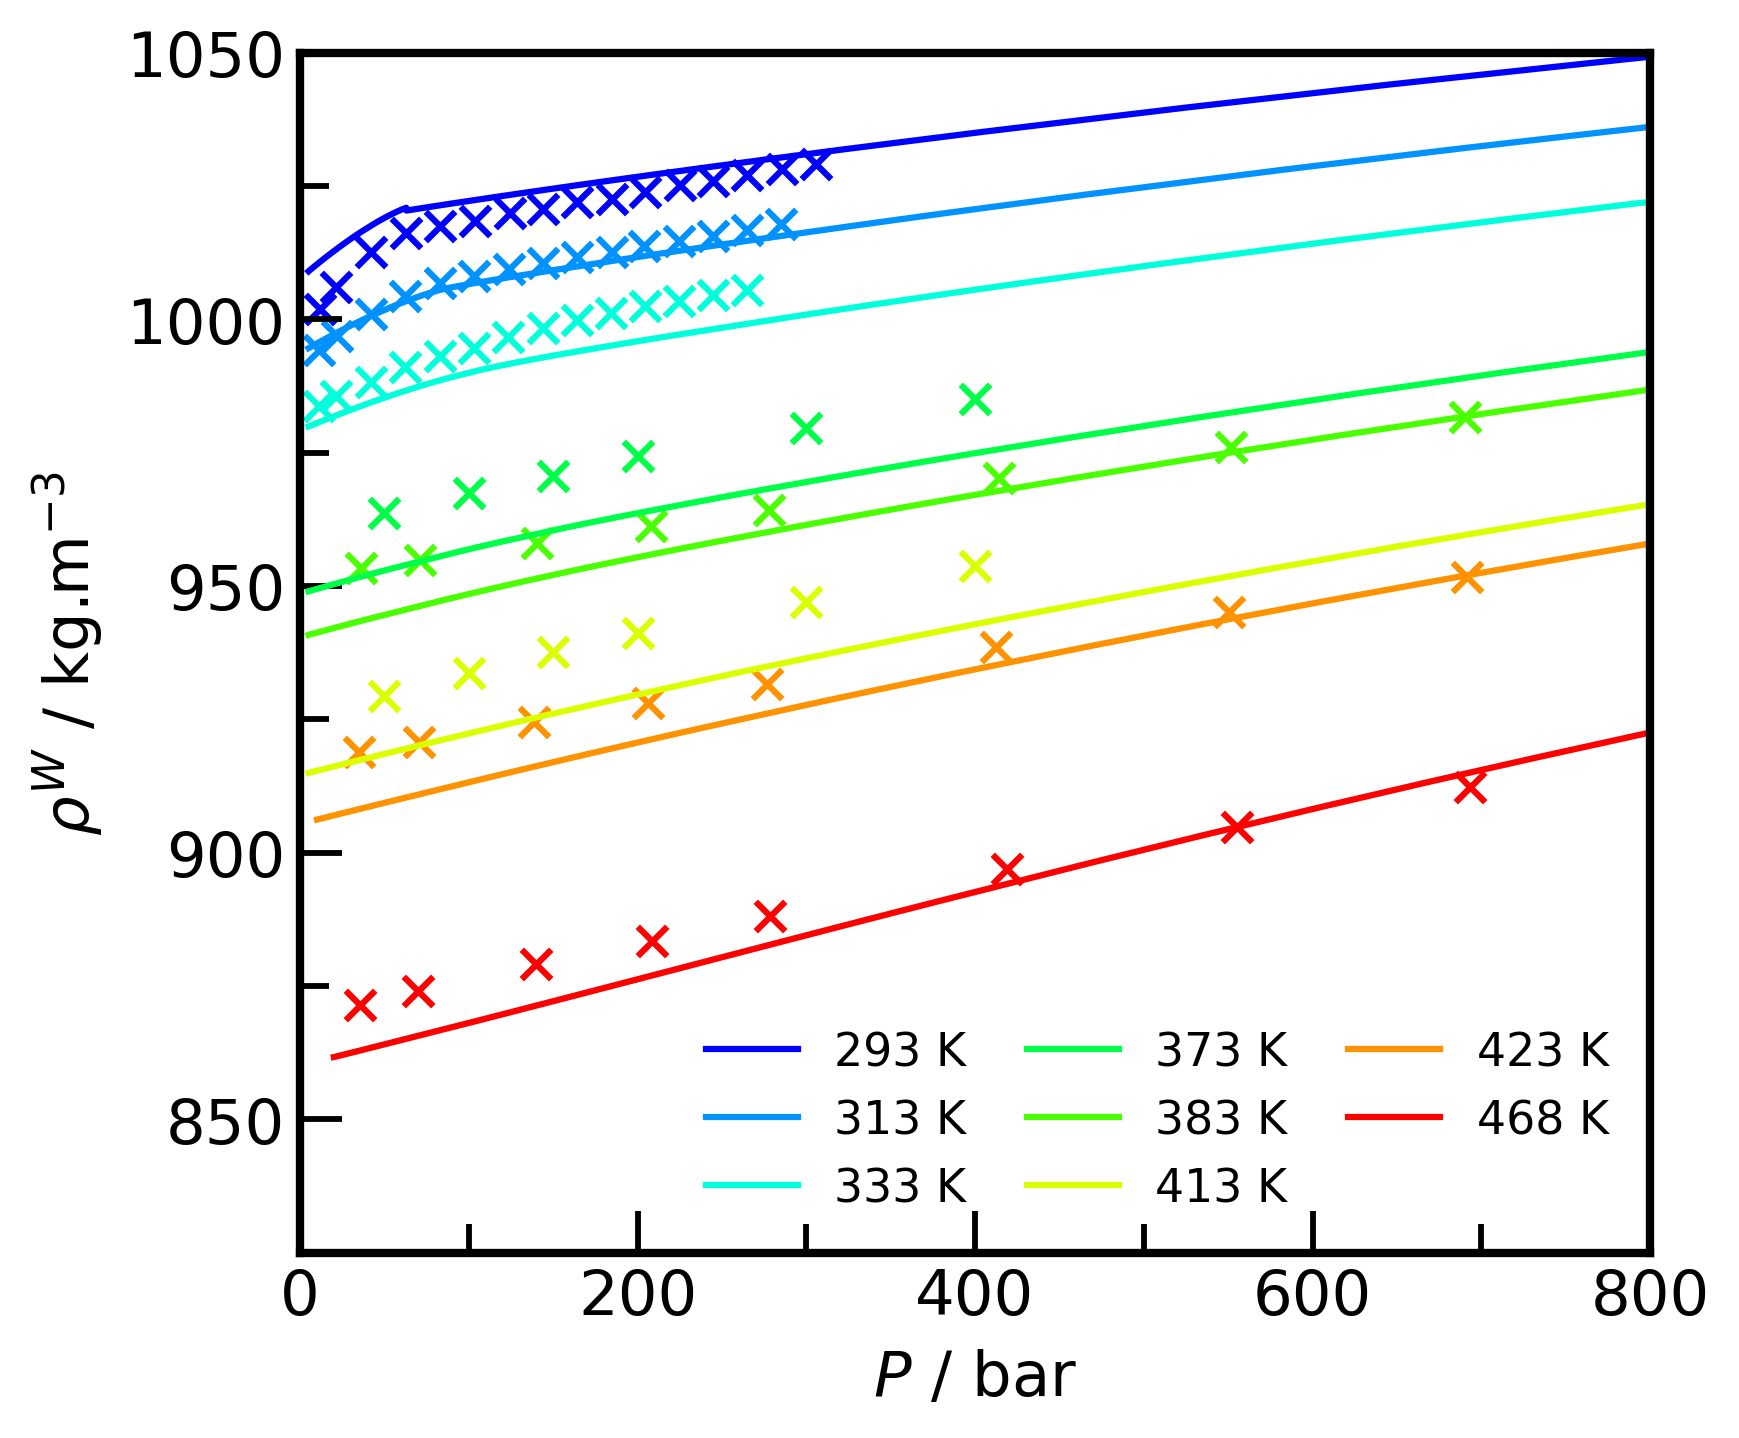
\includegraphics[width=.98\linewidth]{Figures/rhoW_CPAvsEXP.png}
  \caption{ }
\end{subfigure}%
\vskip\baselineskip
\begin{subfigure}{.45\textwidth}
  \centering
  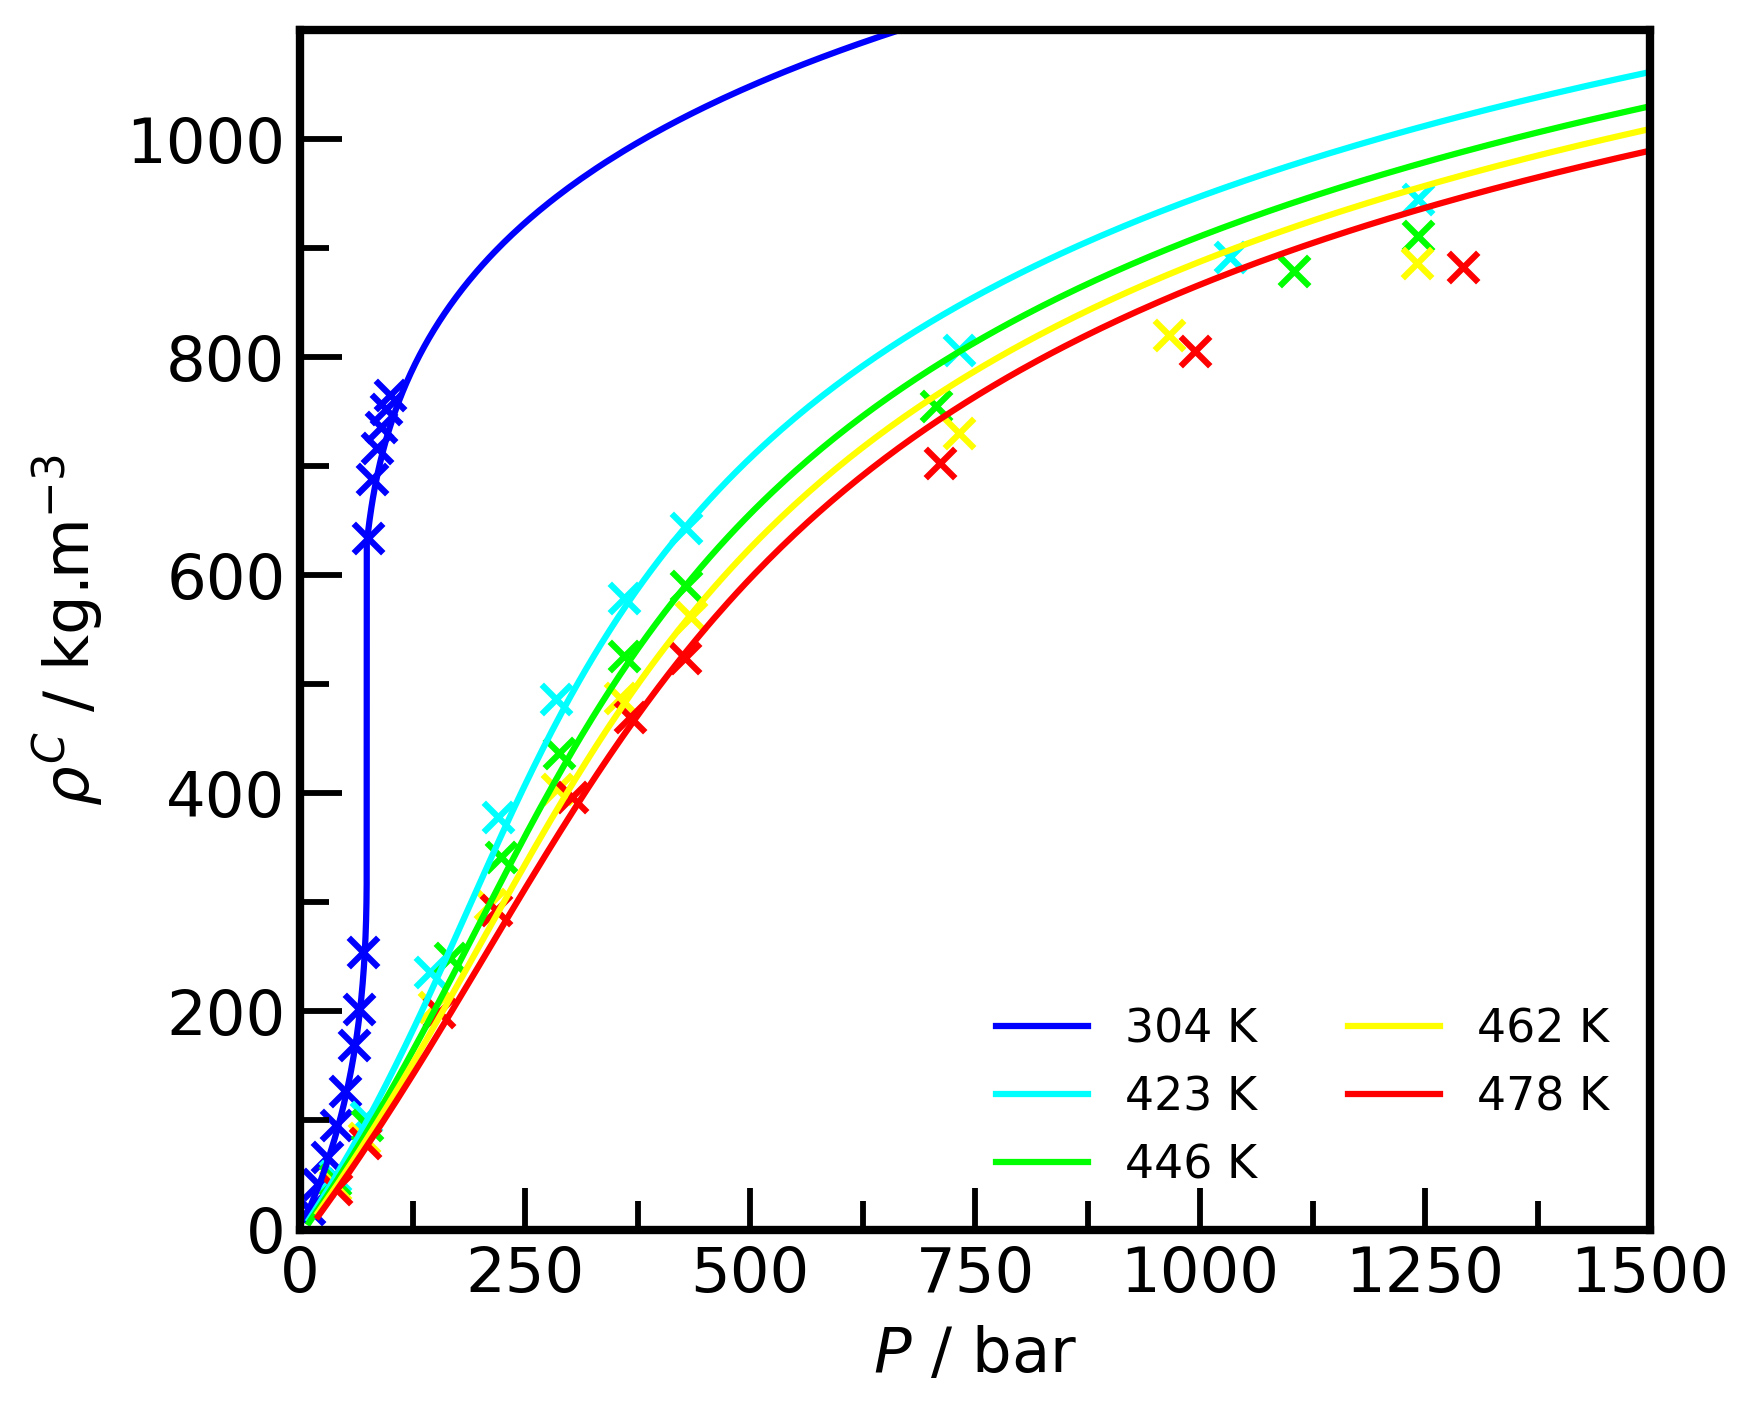
\includegraphics[width=.98\linewidth]{Figures/rhoC_CPAvsEXP.png}
  \caption{ }
\end{subfigure}
\caption{Density of (a) aqueous and (b) \ce{CO2}-rich  phases at equilibrium in the \ce{CO2}-water mixture \textit{vs.} pressure at various temperatures from CPA EoS (continuous line) and experiments \cite{Yan2011, Yaginuma2000, Hebach2004, Tabasinejad2010} (discrete points).} 
\label{RHO_CW}
\end{figure}

The \ce{CO2}-\ce{H2O} phase diagram at high temperatures from the GEMC simulations is shown in Figure \ref{CPAvsGEMC}. At 623 K, the SPCE-EPM2 force field combination predicts a fully miscible mixture in the entire range of pressure and composition. The SPCE critical temperature is estimated at around 623 K \cite{Brovchenko2005}, which implies that both water and \ce{CO2} are supercritical from this temperature. The phase diagrams are very sensitive to the unlike parameters (especially the LJ energy parameter). The phase equilibria are better reproduced by using optimized parameters. Lorentz-Berthelot combining rules are insufficient to describe the contributions of mixing of unlike molecules in the phases \cite{Liu2013} and the unlike parameters may be used as fitting parameters for better results. Overall, the SPCE-EPM2 (OPT) predicts the \ce{CO2}-\ce{H2O} phase diagrams reasonably, especially at 573 K, showing a good transferability of the optimization made by \citeauthor{Vlcek2011} \cite{Vlcek2011}. Oppositely to the CPA EoS, the GEMC simulations are purely predictive since no high-temperature \textcolor{red}{LLE} data is used to adjust parameters. We have not corrected the SPCE overpolarization in the \ce{CO2}-rich phase, indicating that thermal effects overcome the polarization effects at higher temperatures. At 548 K, the water solubility in the \ce{CO2}-rich phase is underestimated, and at even lower temperatures we expect that such deviation increases and selfpolarization correction may be required \cite{Vlcek2011}.   

\begin{figure}[h!]
\centering
  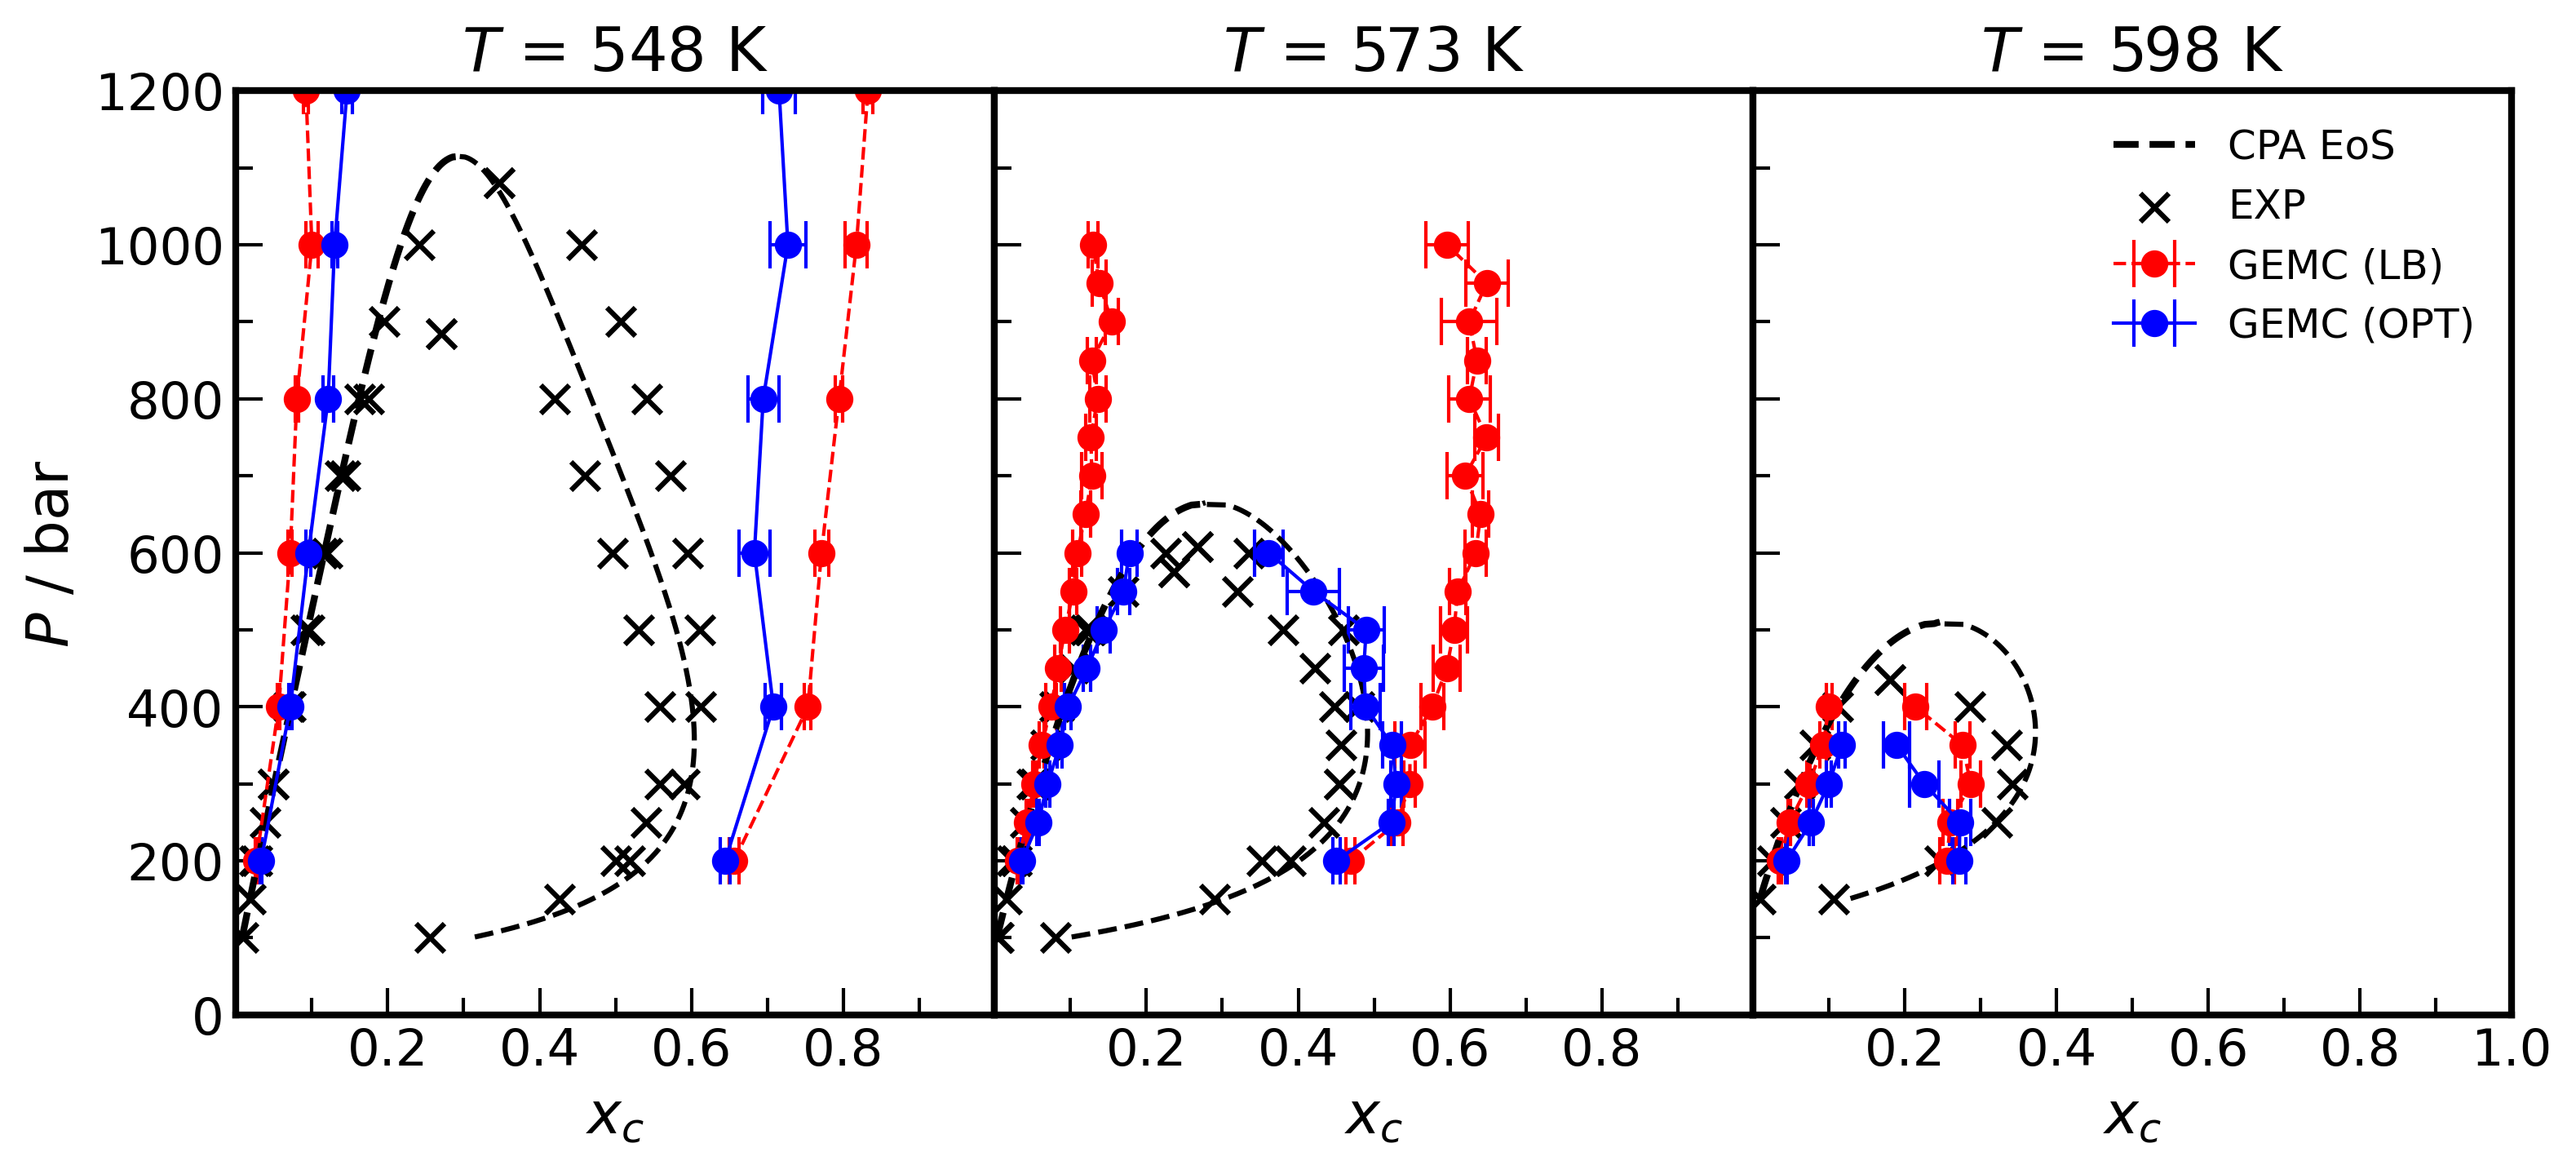
\includegraphics[width=0.85\textwidth]{Figures/GEMCvsEXPvsCPA_CW.png} 
\caption{Phase diagram of \ce{CO2}-\ce{H2O} mixture at $T$ = 548, 573 and 598 K from GEMC simulations, CPA EoS and experiments \cite{Guo2014, Tödheide1963, Takenouchi1964}. ``LB'' and ``OPT'' stand for Lorentz-Berthelot and optimized (at lower temperatures \cite{Vlcek2011}) unlike parameters between \ce{CO2}-\ce{H2O} molecules, respectively.}
\label{CPAvsGEMC}
\end{figure}

The density of the \ce{CO2}-\ce{H2O} phases at equilibrium at high temperature from CPA and GEMC are shown in Figure S6 of the Supporting  Information. Both equation of state and molecular simulations predict a similar trend for the saturated density. The aqueous phase density from GEMC, however, is systematically lower than the CPA. We compare the phase diagrams from our GEMC simulations with SPCE-EPM2 to other classical \cite{Liu2011} and polarizable \cite{Jiang2017a} force field combinations in Figures S7 and S8 of the Supporting Information. The optimized SPCE-EPM2 reproduces the phase diagrams more accurately than other classical force fields (Exp6-Exp6, SPC-EPM2, TIP4P-EPM2, TIP4P2005-Trappe) and provides a similar performance compared to polarizable force field with hydrogen-bonding potential (HBP-GPC). 


\subsection{\ce{CO2}-Brine Mixture}
The \ce{CO2} solubility in brine is obtained from eCPA EoS at high temperatures and NaCl concentration of 6 and 20 weight \% (Figure \ref{ELV_CB_Thigh}). The model captures the nontrivial and nonmonotonic behavior of the solubility trend, including the temperature that gives the maximum solubility for each pressure. Figure S9 of the Supporting Information shows the \ce{CO2} solubility in brine at lower temperatures ($T$ < 500 K). An excellent agreement with experiments is found for temperatures higher than 298 K. The trend with temperature is incorrect at $T$ < 298 K, which indicates that the model may not describe solubility at very low temperatures.  In the entire range of temperature (283 — 723 K) and pressure (1 — 1400 bar), the absolute average deviation is 6.9\% for \ce{CO2} solubility in brine (Table \ref{EXPs_CW}).  

\begin{figure}[h!]
\centering
  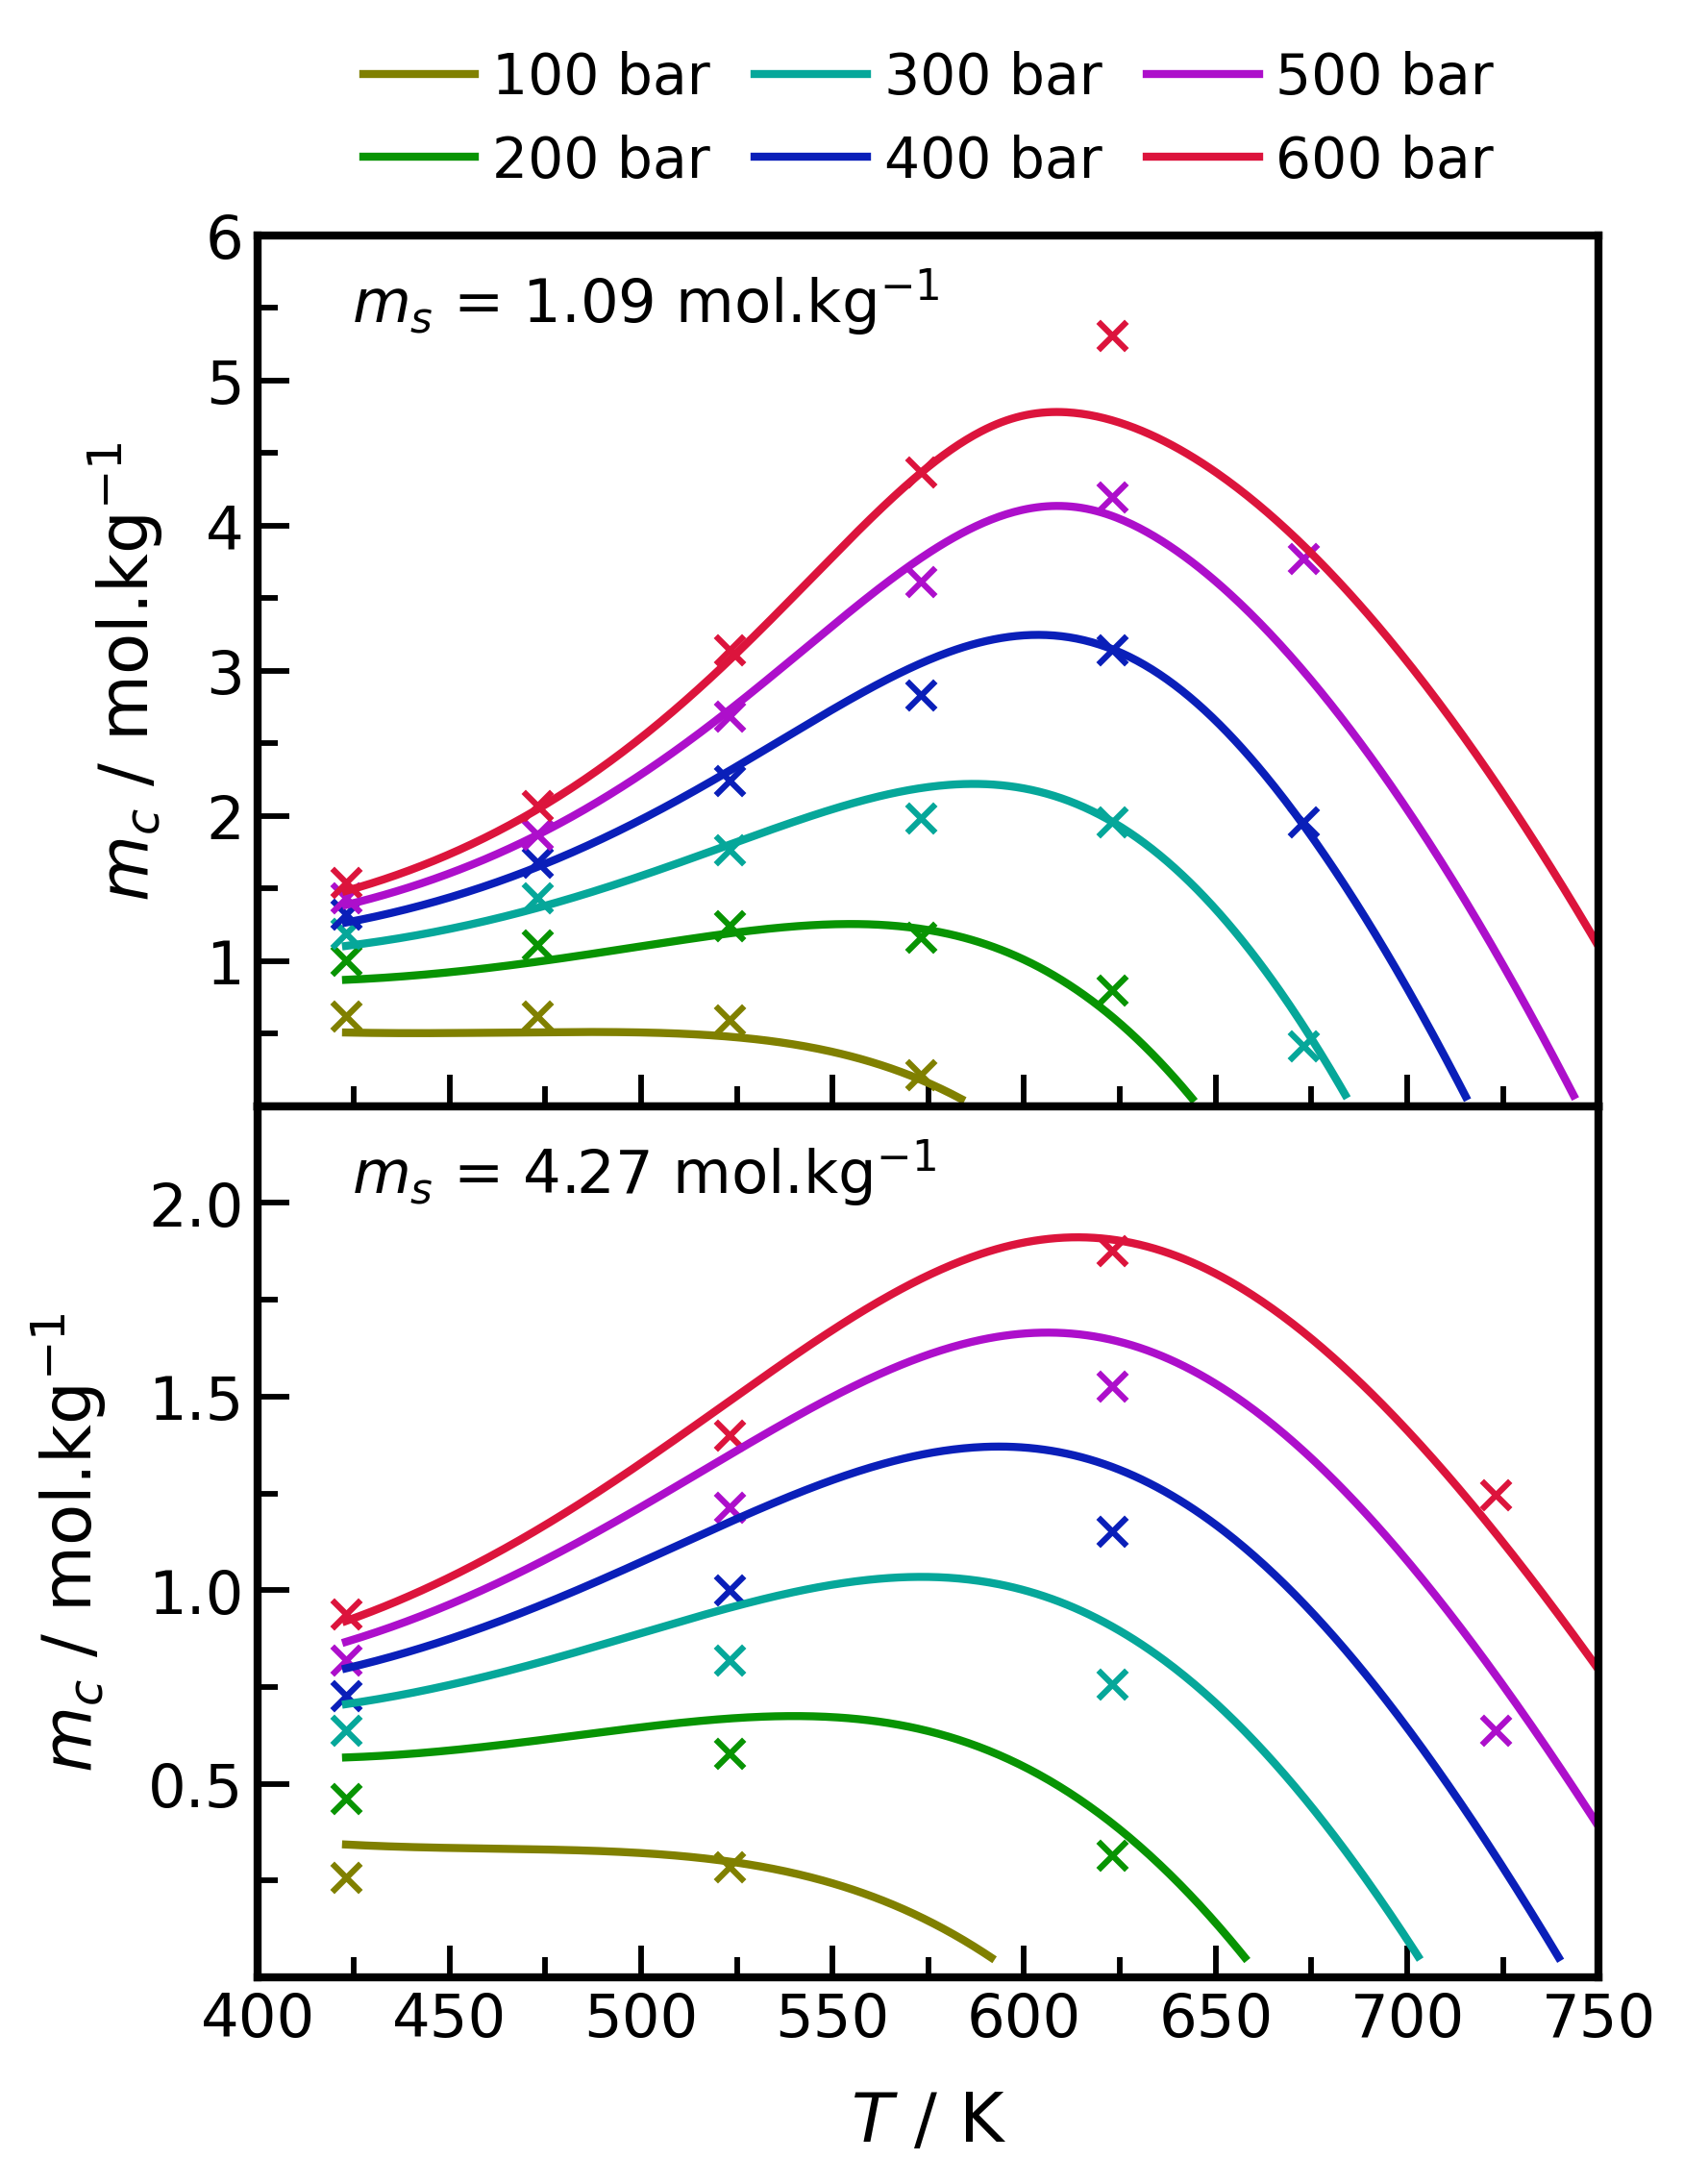
\includegraphics[width=0.5\textwidth]{Figures/eCPA_Thigh.png} 
\caption{\ce{CO2} solubility in NaCl brine at high temperature ($T$ > 423 K)  from eCPA EoS (continuous line) and experiments \cite{Takenouchi1965} (discrete points) for various pressures and salinities of 1.09 and 4.27 mol$\cdot$kg$^{-1}$ (6 and 20 wt\%, respectively) }
\label{ELV_CB_Thigh}
\end{figure}

Figure S10 of the Supporting Information compares our model to the eCPA from \citeauthor{Maribo2015} \cite{Maribo2015}.  \textcolor{red}{Using the same experimental data set, the absolute average deviation of the eCPA EoS by \citeauthor{Maribo2015} \cite{Maribo2015} and by this work are estimated to be 26.6\% and 6.9\%, respectively. The \ce{CO2} solubility in brine is improved by 74\% with our model.} In general, our eCPA better reproduces the experimental data in the entire range of conditions, showing significant deviations only at very high pressures ($P$ > 1000 bar).  The major difference between the two is the \ce{CO2}-\ce{H2O} cross-association, which is only accounted for in our work, indicating the importance of such interactions in the modeling of \ce{CO2} in aqueous mixtures. Another key factor for our model high accuracy is the consideration of temperature-dependent interaction parameters. The solubility dependency on temperature in mixtures containing acid gases and water is nontrivial and would be limited for a narrow range of conditions if temperature-independent parameters are chosen \cite{Tsivintzelis2011}.  

The density of the \ce{CO2}-saturated brine is computed with eCPA (Figure \ref{RHO_CB}.a). The trends with temperature, pressure, and salinity are reproduced with an average absolute deviation of 1.05\%. We compute the density of unsaturated brine solutions at various \ce{CO2} concentrations (Figure S11 of the Supporting Information). \citeauthor{Song2013} \cite{Song2013} have reported experimental brine density with \ce{CO2} concentration up to 3 wt\%, which is above the \ce{CO2} equilibrium concentration for certain conditions. We use for comparison only data below the saturation point. In the range of 333 to 413 K, 100 to 180 bar, and 1 to 4 m, our eCPA EoS gives an average absolute deviation of 1.10\% for unsaturated solutions. Similar to the \ce{CO2}-water mixture, no experimental density data are available for the \ce{CO2}-brine mixture at higher temperatures.   

\begin{figure}[h!]
\begin{subfigure}{.61\textwidth}
  \centering
  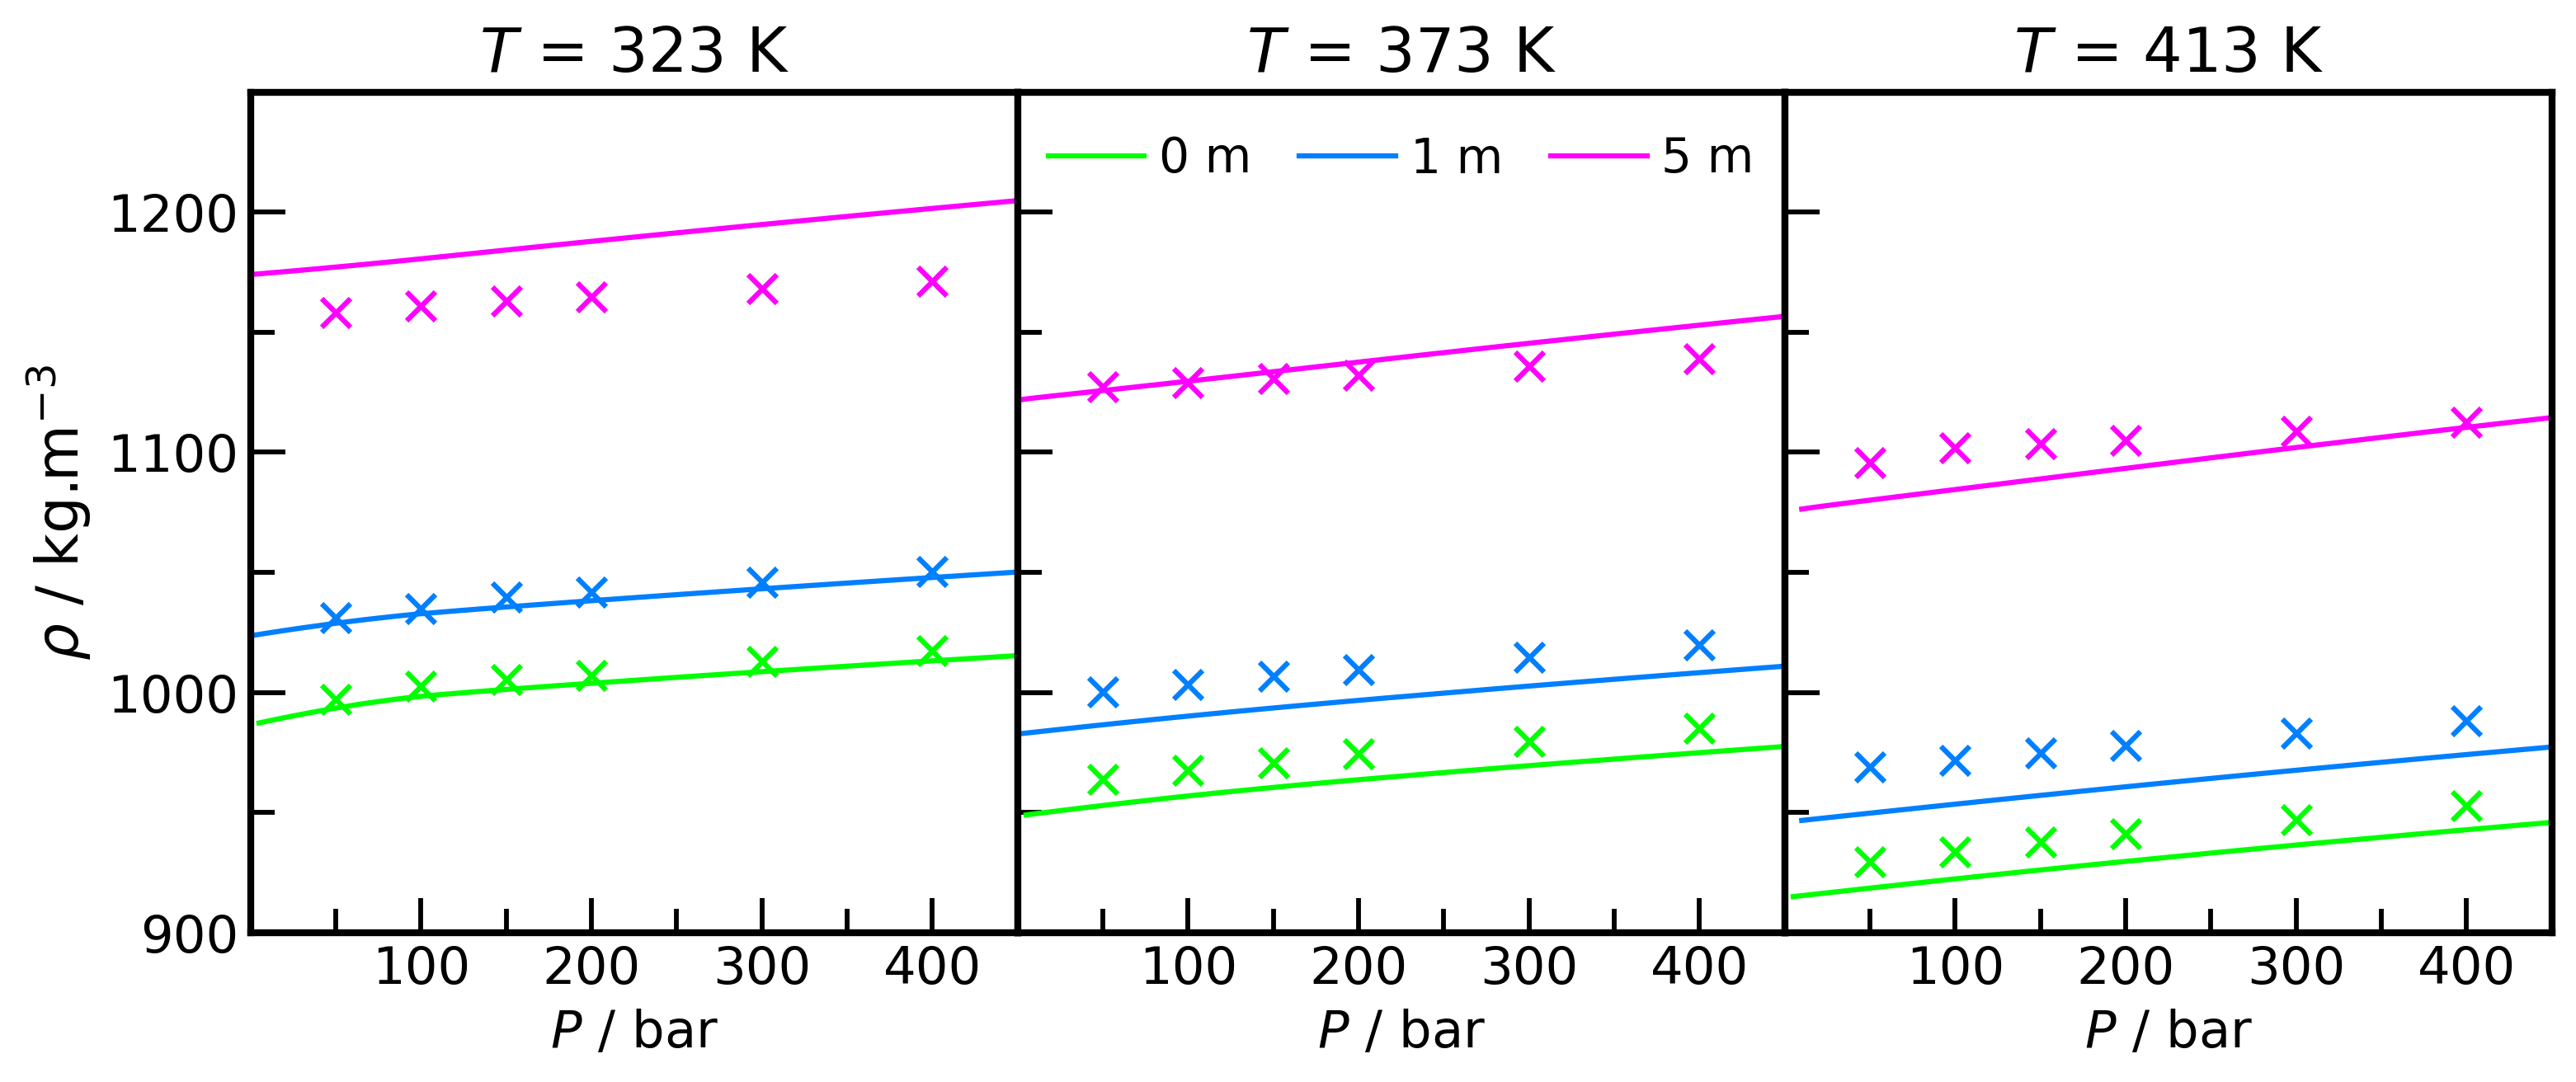
\includegraphics[width=.98\linewidth]{Figures/rhoW_CB.png}
  \caption{ }
\end{subfigure}%
\begin{subfigure}{.36\textwidth}
  \centering
  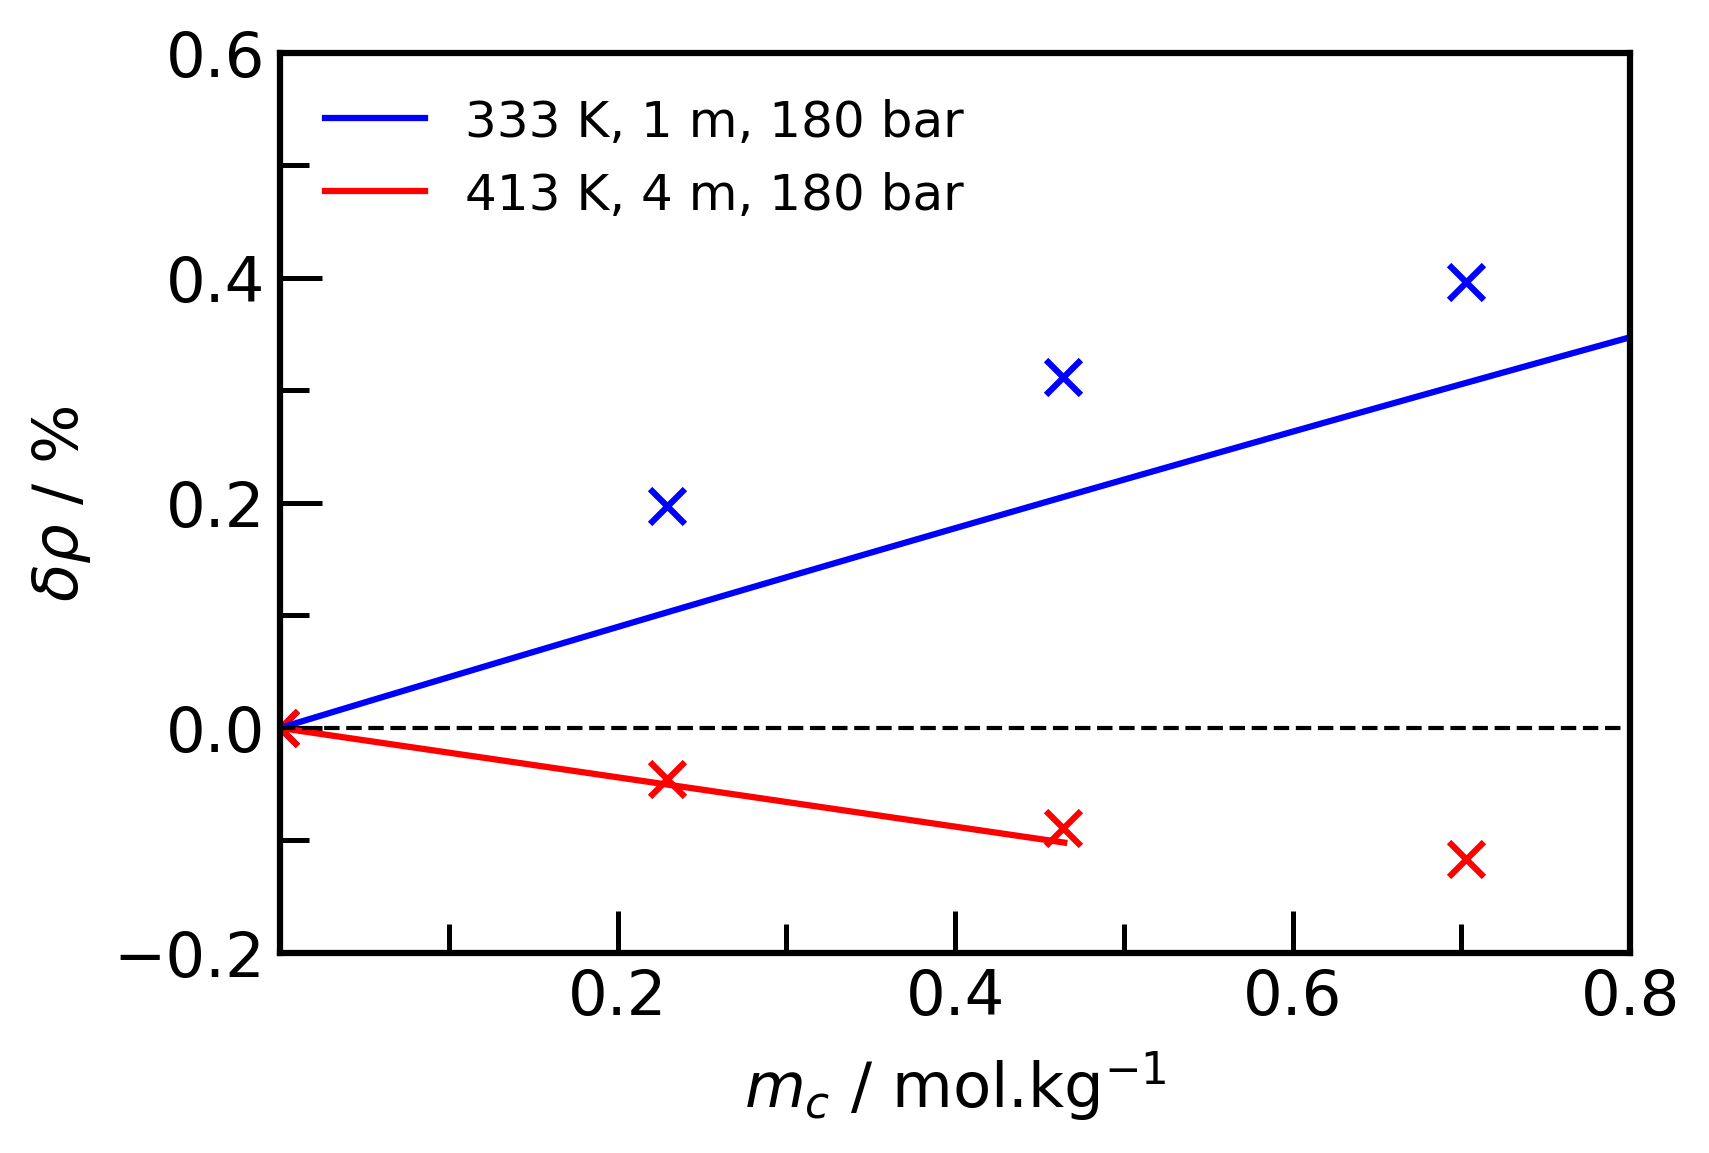
\includegraphics[width=.98\linewidth]{Figures/DeltaRho_msT.png}
  \caption{ }
\end{subfigure}
\caption{(a) Density of \ce{CO2}-saturated NaCl brine \textit{vs.} pressure at various temperatures and salinities from eCPA EoS (continuous line) and experiments \cite{Yan2011} (discrete points). (b) Relative density variation of the unsaturated brine \textit{vs.} \ce{CO2} concentration  ($\delta \rho = (\rho - \rho_{m_c=0})/\rho_{m_c=0})$) at two different conditions from eCPA (continuous line) and experiments \cite{Song2013} (discrete points).} 
\label{RHO_CB}
\end{figure}

Different from the \ce{CO2}-water mixture, \ce{CO2} dissolution may increase or decrease the aqueous phase density in the \ce{CO2}-brine system. Figure \ref{RHO_CB}.b shows the variation of density at two different conditions. At higher salinity and temperature, the aqueous mixture density decreases, which is reproduced by our eCPA EoS. Electrolytes may decrease the \ce{CO2}-\ce{H2O} interactions, increasing \ce{CO2} partial molar volume \cite{Song2013}. \citeauthor{Lu2009} \cite{Lu2009} have shown that for a given pressure and salinity, there is a temperature at which the density becomes independent of the \ce{CO2} concentration; by increasing salinity, the ``equal density temperature'' decreases. A similar effect is observed in the \ce{CO2}-brine thermodiffusion, in which salinity decreases the thermodiffusion inversion temperature for \ce{CO2} migrating to thermophobic to thermophilic \cite{Coelho2023}. These effects shed light on the impact of salinity on the structure and dynamics in the \ce{CO2} aqueous mixture, which should be accounted for accurate modeling of geological formations. 

The salting-out effect is observed in both GEMC simulations and eCPA Eos (Figure \ref{eCPAvsGEMC}). Ions modify the solvation free energy of \ce{CO2}, making it less favorable \cite{Blazquez2024}. The \ce{CO2} solubility reduction with salinity may be slightly overestimated in our GEMC simulations due to the use of integer charges for ions, which leads to an excessive repulsion between \ce{CO2} and electrolytes. Scaled charges may improve the salting-out predictions \cite{Blazquez2024}. Similar results are obtained for LB and OPT unlike parameters, with \ce{CO2} solubility being slightly higher with OPT parameters. In the \ce{CO2}-rich phase, the water solubility decreases with salinity (Figure S12 of the Supporting Information). The presence of ions increases the range of conditions in which the mixture is immiscible. The saturated aqueous density difference observed between GEMC and CPA (Figure S6 of the Supporting Information) vanishes by increasing salinity (Figure S13 of the Supporting Information). The increase in brine density with salt concentration is higher by the GEMC simulations than by the eCPA EoS, which can be again due to the use of integer electrolyte charges that overestimates the ionic association \cite{Coelho2024}.  


\begin{figure}[h!]
\centering
  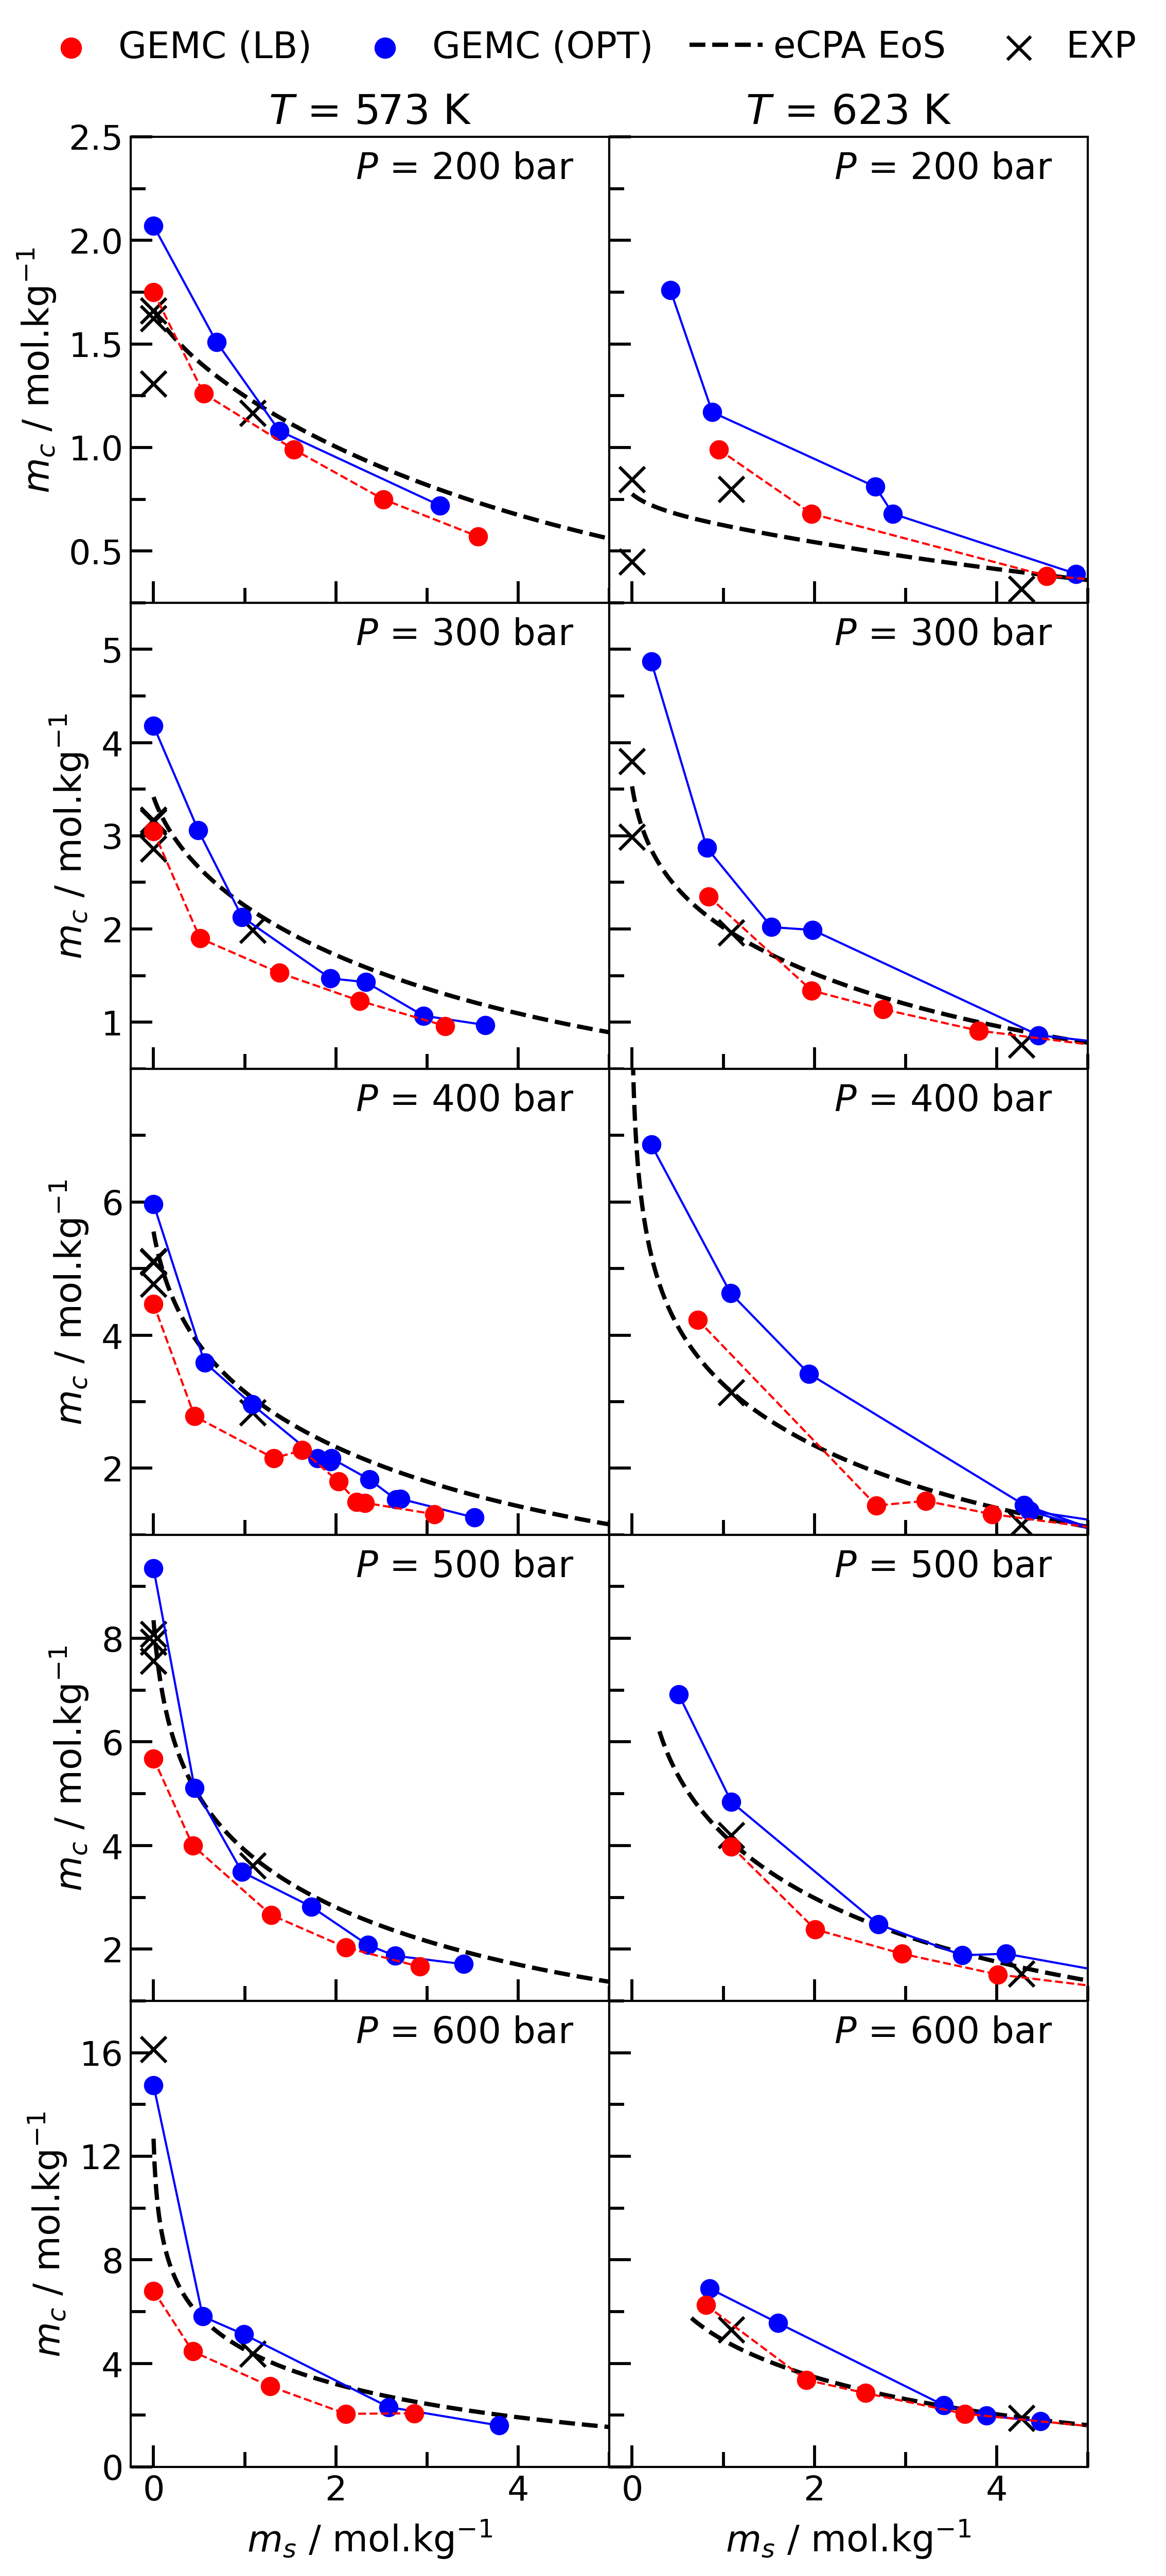
\includegraphics[width=0.5\textwidth]{Figures/GEMCvseCPAvsEXP_LBvsVC.png} 
\caption{\ce{CO2} solubility in NaCl brine \textit{vs.} salt concentration at various pressures and two different temperatures from GEMC simulations, eCPA EoS and experiments \cite{Guo2014, Tödheide1963, Takenouchi1965}. ``LB'' and ``OPT'' stand for Lorentz-Berthelot and optimized (at lower temperatures \cite{Vlcek2011}) unlike parameters between \ce{CO2}-\ce{H2O} molecules, respectively.}
\label{eCPAvsGEMC}
\end{figure}

\subsection{Association}

Association and cross-association are important aspects of the structure of \ce{CO2}-water and \ce{CO2}-brine mixtures. From EoS, the non-bonded fraction of associating molecules ($\chi_i$) provides insights into the fluid-structure. From molecular simulations, the radial distribution function ($g_{ij}(r)$) and the coordination number ($n^{ij}$) between atoms are direct alternatives to investigate structures. Water self-association is represented by hydrogen bonds (O$_w$-H$_w$). \ce{CO2}-water cross-association can either be by hydrogen bonds (O$_c$-H$_w$) or tetrel bonds (O$_w$-C$_c$) as shown in Figure S14 of the Supporting Information. \ce{CO2}-water hydrogen bonds are short-lived and may be less stable than tetrel bonds \cite{Glezakou2010}. A similar phenomenon has been reported for \ce{CO2}-\ce{H2S} mixture \cite{Gonçalves2022}.

By geometrically defining hydrogen bonds as O-H pairs at separations less than 2.45 \AA \cite{Vlcek2011, Dufal2015}, we can compute them directly from the radial distribution functions. A cross-association through tetrel bonds requires information on the angle between molecules. To compare with the EoS, we assume the probability of cross-association through hydrogen bonds or tetrel bonds to be the same, and compute only the hydrogen bond. The number of hydrogen bonds of each interaction per molecule and the non-bonded fraction of molecules from molecular simulations are given by \cite{Dufal2015}:
\begin{equation}
    n^{\text{O}_w\text{H}_w} = \frac{N_{\text{H}_w}}{2V}\int\limits_0 ^{r_c} g_{\text{O}_w\text{H}_w}(r) 4 \pi r^2 \mathrm{d}r, 
    \label{OwHw}
\end{equation}
\begin{equation}
    n^{\text{O}_c\text{H}_w} = \frac{N_{\text{H}_w}}{V}\int\limits_0 ^{r_c} g_{\text{O}_c\text{H}_w}(r) 4 \pi r^2 \mathrm{d}r,
    \label{OcHw}
\end{equation}
\begin{equation}
    \chi_w = 1 -  n^{\text{O}_w\text{H}_w} - \frac{N_{\text{O}_c}}{N_{\text{H}_w}} n^{\text{O}_c\text{H}_w},
    \label{chiw_MD}
\end{equation}
\begin{equation}
    \chi_c = 1 - n^{\text{O}_c\text{H}_w},
    \label{chic_MD}
\end{equation}
where $V$ is the volume, $N_i$ is the number of atoms $i$ in the simulation box and $r_c$ is the hydrogen bond cutoff (2.45 \AA). Each water-oxygen has two associating sites, whereas each \ce{CO2}-oxygen has one. We perform molecular dynamics (MD) simulations to determine the radial distribution functions and non-bonded associating fractions for each condition.

Figure \ref{Structure} shows the association and cross-association in the \ce{CO2}-water (\ref{Structure}.a) and \ce{CO2}-brine (\ref{Structure}.b) mixtures from MD and EoS. We use OPT unlike parameters for the MD simulations, but the association and cross-association are about the same with LB parameters (Figure S15 of the Supporting Information). Although MD and EoS are completely different techniques that have been parametrized with different datasets, they predict very similar association structures for water and \ce{CO2}. The trends with pressure, temperature and salinity are in good agreement for water molecules. The \ce{CO2} cross-association with salinity increases from MD simulations but slightly decreases from eCPA EoS. Nevertheless, they still have the same order of magnitude. From a molecular simulation perspective, we can advocate for the use of \ce{CO2}-\ce{H2O} cross-association. 

By defining the association ratio as the ratio between the number of associating \ce{CO2}  and the number of associating \ce{H2O} molecules, we can quantify how significant is cross-association related to water association (Figure S16 of the Supporting Information). The association ratio from the equation of state is higher than that from MD simulations.  In the \ce{CO2}-rich phase, although the fraction of associating \ce{CO2} is small ($\chi_c \approx 1$), the association ratio is an order of magnitude higher than in the aqueous phase. Cross-association is as significant as water self-association in non-polar environments \cite{Li2009} and should be accounted for properly in the modeling. 
%once the fraction of associating \ce{CO2} molecules can be up to 40 \%. 

\begin{figure}[h!]
\begin{subfigure}{.43\textwidth}
  \centering
  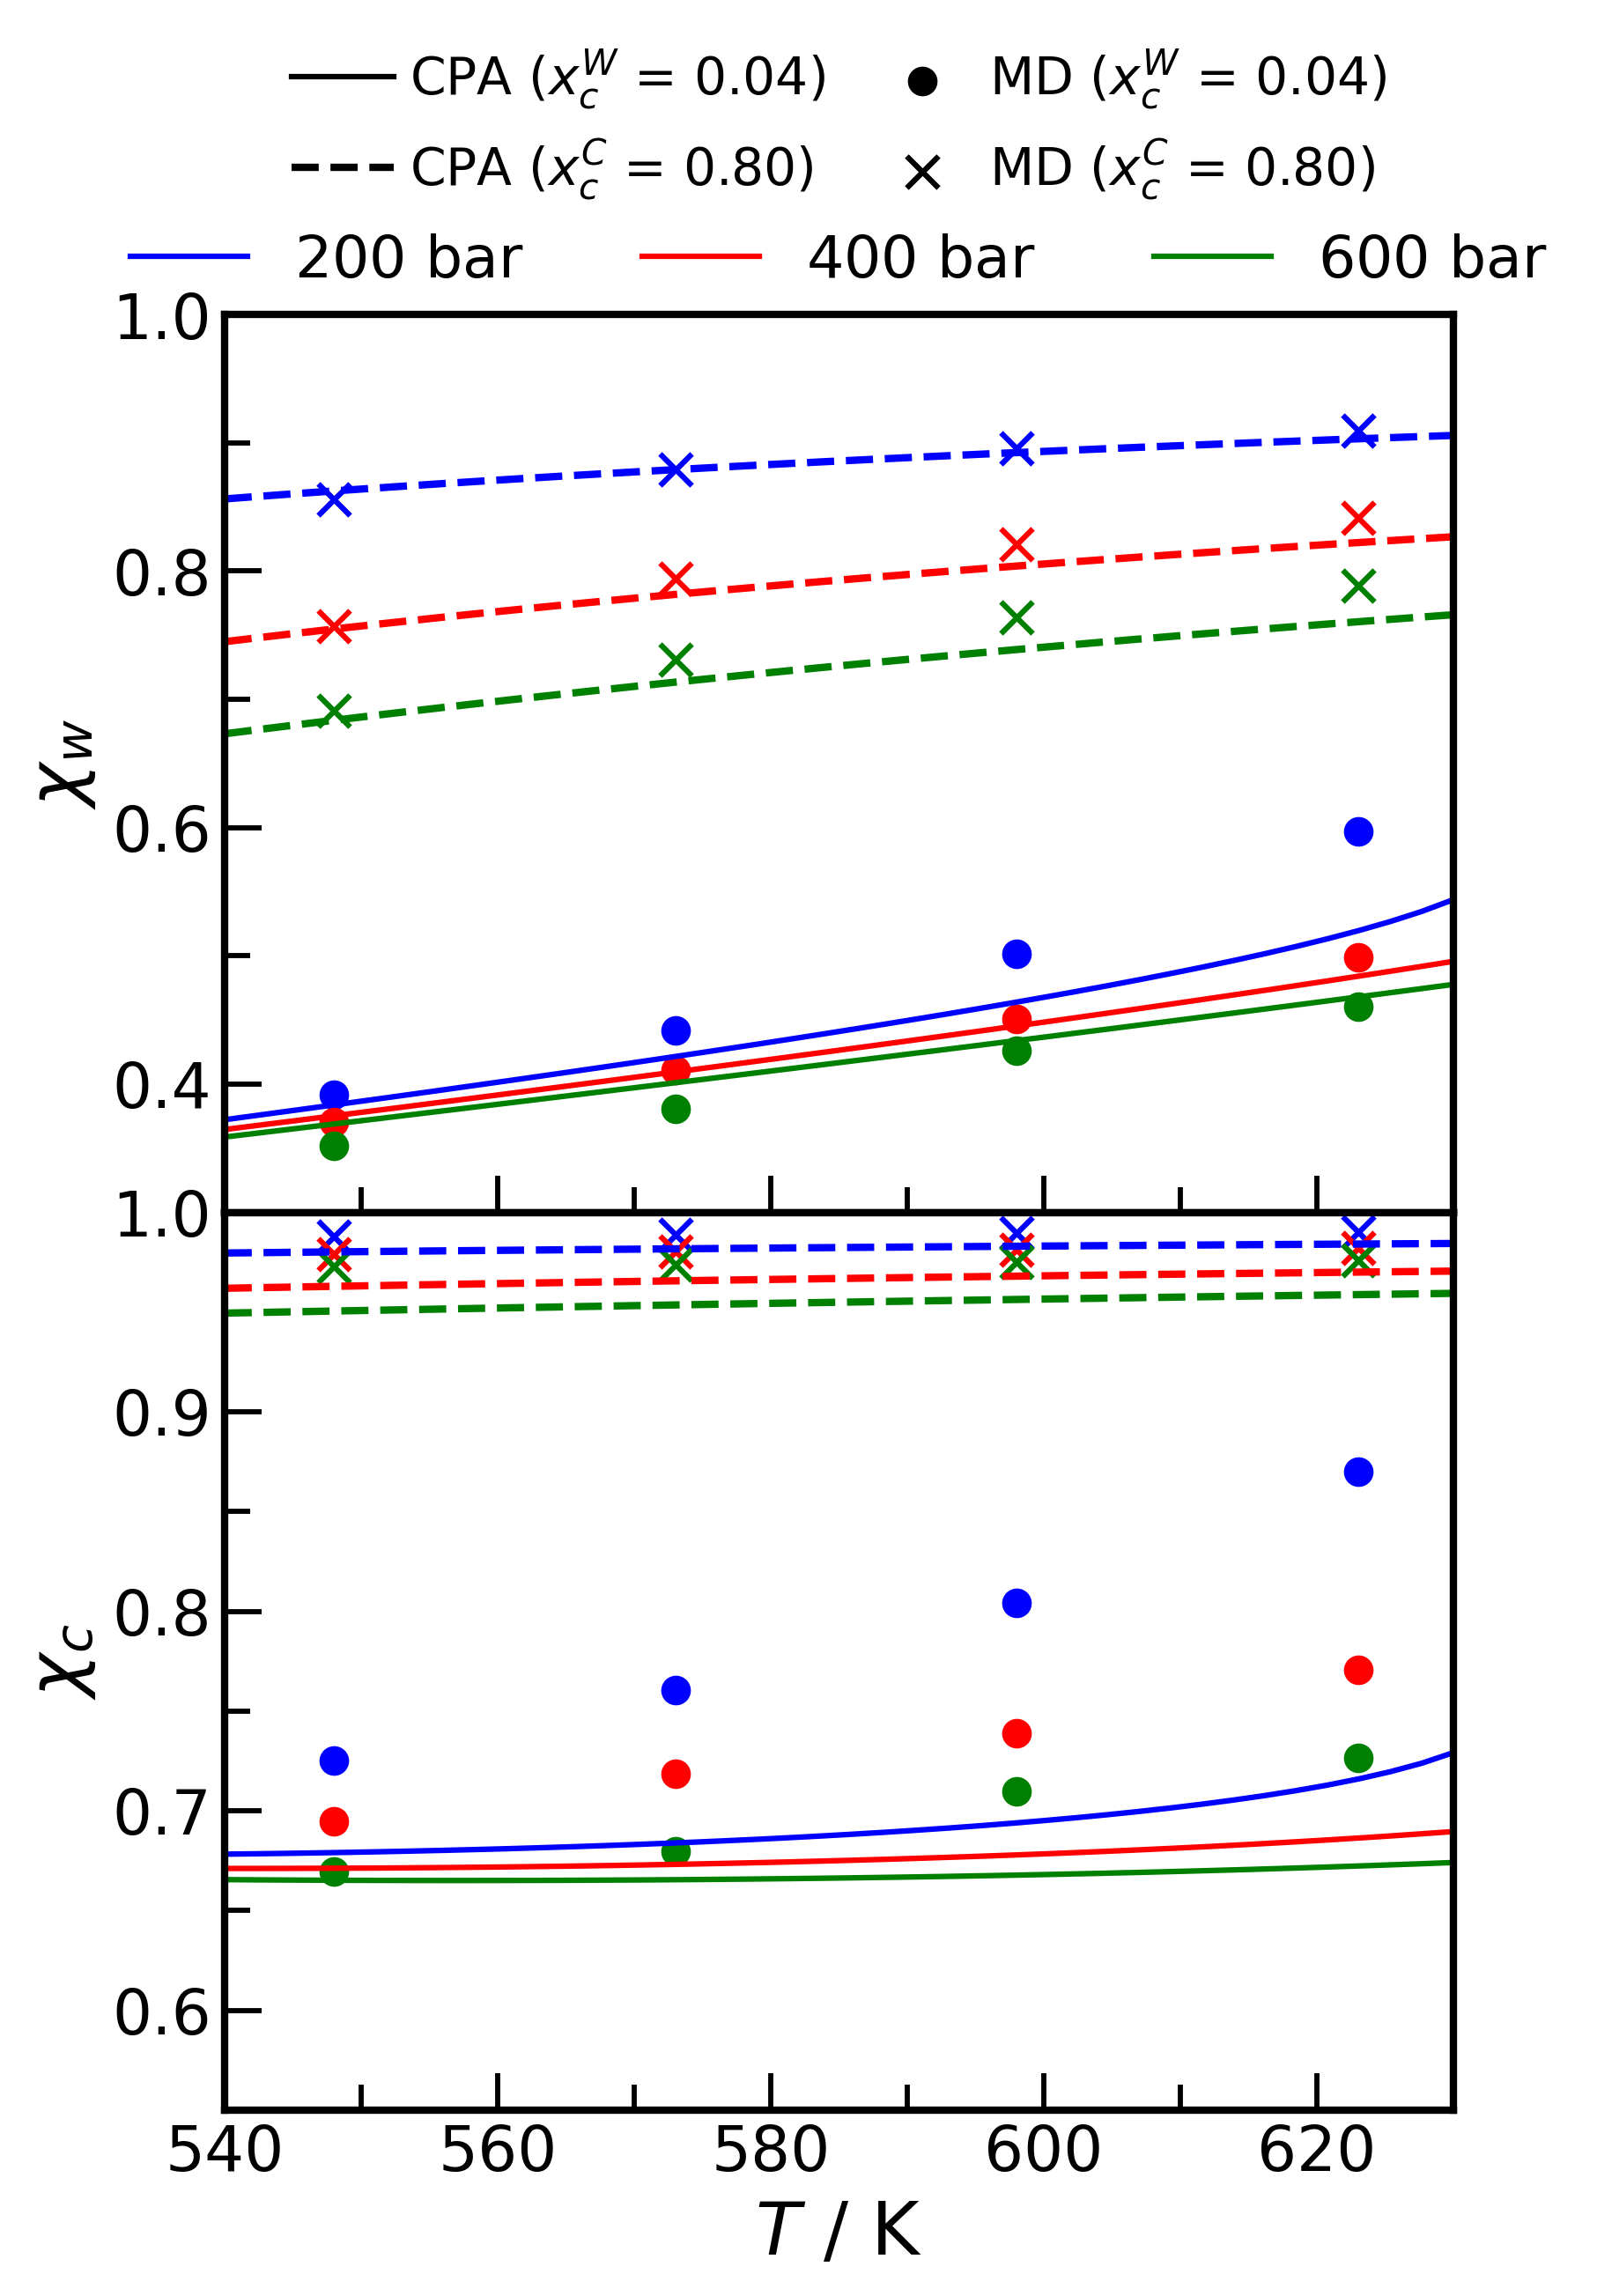
\includegraphics[width=.98\linewidth]{Figures/CW_Structure.png}
  \caption{ }
\end{subfigure}%
\begin{subfigure}{.56\textwidth}
  \centering
  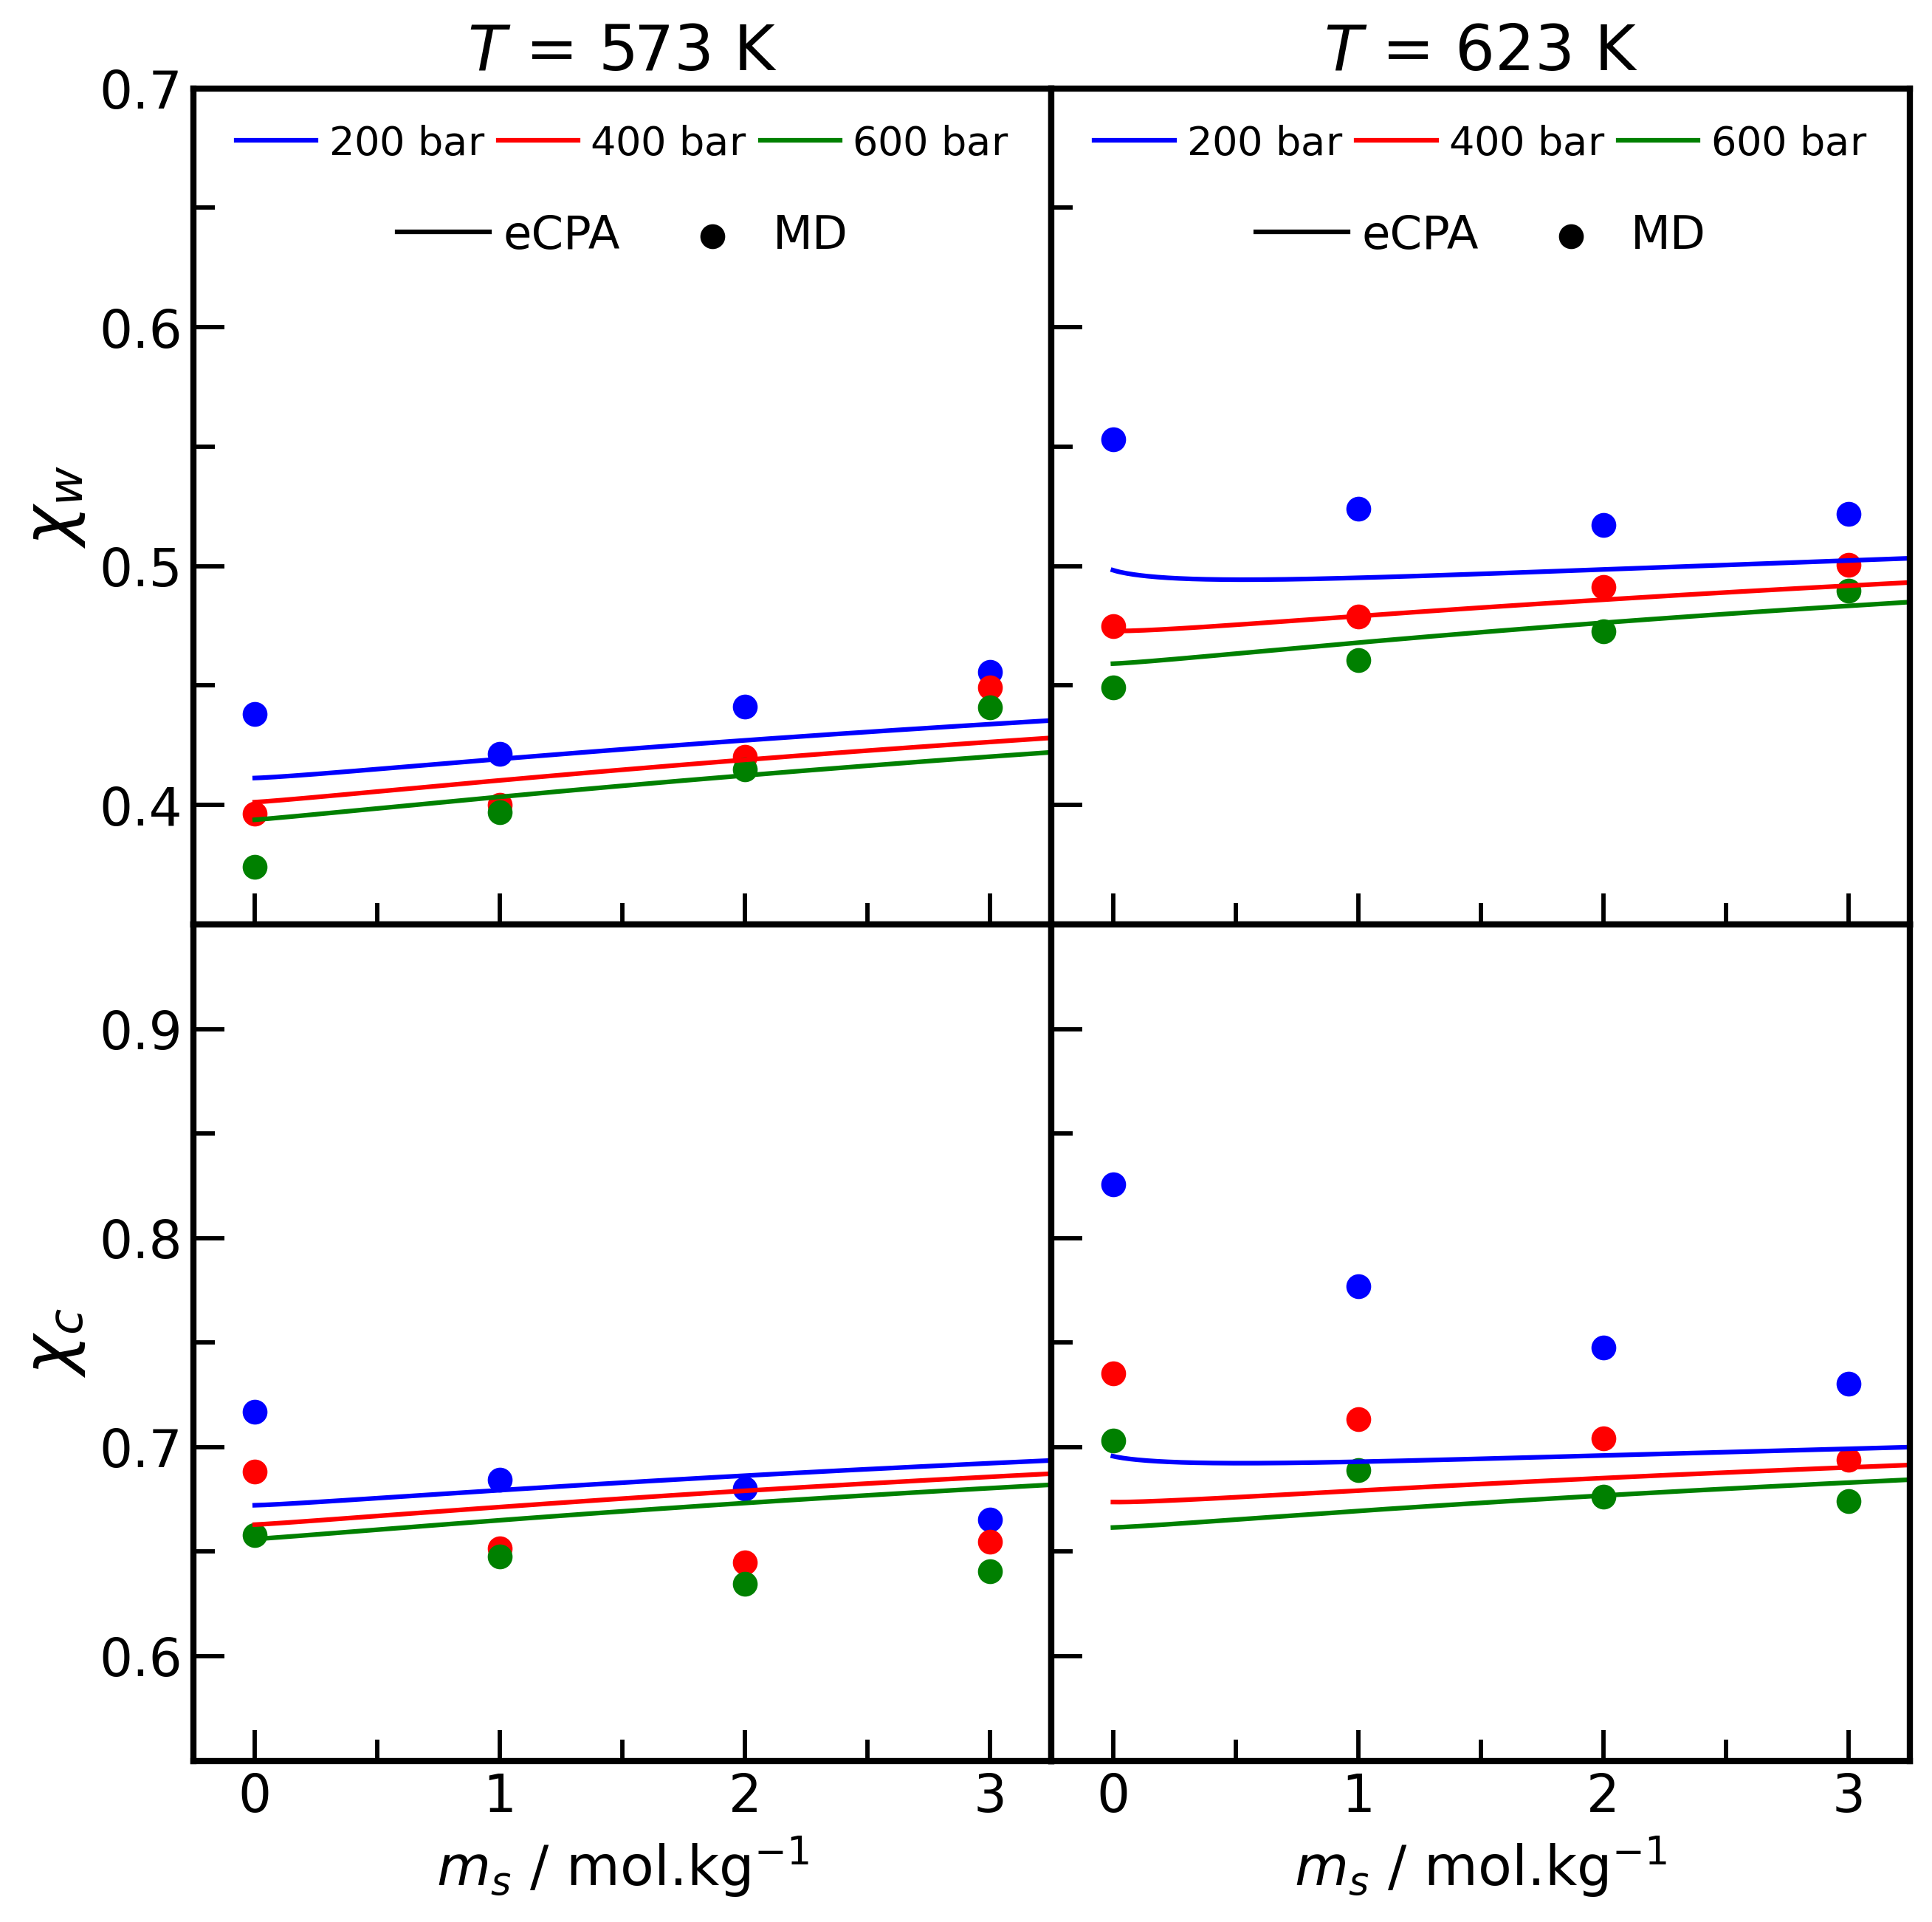
\includegraphics[width=.98\linewidth]{Figures/CB_Structure.png}
  \caption{ }
\end{subfigure}
\caption{Association ($\chi_w$) and cross-association ($\chi_c$) in the \ce{CO2}-water and \ce{CO2}-brine mixtures from MD simulations (discrete points) and CPA/eCPA EoS (continuous line). (a) Non-bonded fractions \textit{vs.} temperature in the \ce{CO2}-water mixture at $x_c$ = 0.04 (aqueous phase) and 0.80 (\ce{CO2}-rich phase) and various pressures. (b) Non-bonded fractions \textit{vs.} salt concentration in the \ce{CO2}-brine mixture at $x_c$ = 0.02 and various pressures and temperatures.} 
\label{Structure}
\end{figure}

